\chapter{CONSTANT pH MOLECULAR DYNAMICS IN EXPLICIT SOLVENT}

In this chapter, I present a new method for performing CpHMD simulations in
explicit solvent building on the discrete protonation state model developed and
explained in Ch. \ref{ch3}.

\section{Introduction}

Recently, \citeauthor{Machuqueiro_Proteins_2011_v79_p3437} raised concerns about
pK\sub{a} predictions inheriting problems related to the model compound
definition and inaccuracies in the underlying force field.
\cite{Machuqueiro_Proteins_2011_v79_p3437} In particular, force field
deficiencies have been shown to result in incorrect---even unphysical---global
minima. \cite{Zgarbova_JChemTheoryComput_2011_v7_p2886,
Cheatham_Biopolymers_2001_v56_p232, Varnai_NucleicAcidsRes_2002_v30_p5398,
Hornak_Proteins_2006_v65_p712, Klepeis_CurrOpinStructBiol_2009_v19_p120}
\citeauthor{Machuqueiro_Proteins_2011_v79_p3437}'s work suggests that pK\sub{a}
predictions are improved when the sampled conformations more closely resemble
the true, experimental ensemble. Therefore, the role of GB in evaluating the
dynamics of biomolecules may be problematic in certain situations where GB is
known to fail, such as the over-stabilization of salt bridges.
\cite{Zhou_Proteins_2003_v53_p148, Geney_JChemTheoryComput_2006_v2_p115} Indeed,
for highly charged systems, like nucleic acids, a more accurate treatment of
electrostatic interactions is required to build a sensible ensemble.

While most of the physics-based methods designed to describe a biomolecular
system at constant pH use an implicit solvent representation of the solvent,
several CpHMD methods have been extended to sample, at least conformations, in
explicit solvent with both the discrete 
\cite{Baptista_JChemPhys_2002_v117_p4184} and continuous 
\cite{Donnini_JChemTheoryComput_2011_v7_p1962,
Wallace_JChemTheoryComput_2011_v7_p2617, Goh_JChemTheoryComput_2012_v8_p36}
protonation models.  The methods proposed by
\citeauthor{Baptista_JChemPhys_2002_v117_p4184}
\cite{Baptista_JChemPhys_2002_v117_p4184} and
\citeauthor{Wallace_JChemTheoryComput_2011_v7_p2617}
\cite{Wallace_JChemTheoryComput_2011_v7_p2617} use an implicit solvent
potential to sample protonation states while the methods developed by
\citeauthor{Goh_JChemTheoryComput_2012_v8_p36}
\cite{Goh_JChemTheoryComput_2012_v8_p36} and
\citeauthor{Donnini_JChemTheoryComput_2011_v7_p1962} 
\cite{Donnini_JChemTheoryComput_2011_v7_p1962} perform $\lambda$-dynamics on the
titration coordinate directly in explicit solvent. A more recent approach by
\citeauthor{Wallace_JChemPhys_2012_v137_p184105} uses a $\lambda$-dynamics
approach in pure explicit solvent, but adds a counter-ion whose charge is
changed simultaneously with a titratable residue in order to maintain charge
neutrality in the unit cell. \cite{Wallace_JChemPhys_2012_v137_p184105}

Discrete protonation methods use molecular dynamics to propagate the spatial
coordinates, while occasionally interrupting the dynamics to attempt change(s)
to the protonation states of the titratable residues using a Metropolis Monte
Carlo criteria. The CpHMD method implemented in Amber
\cite{Mongan_JComputChem_2004_v25_p2038} (and later implemented in CHARMM
\cite{Itoh_Proteins_2011_v79_p3420}) performs MD in GB solvent, periodically
attempting to change the protonation state of one or two interacting residues
roughly every 10 fs. \cite{Mongan_JComputChem_2004_v25_p2038} In the stochastic
titration method described by \citeauthor{Baptista_JChemPhys_2002_v117_p4184},
dynamics is run in explicit solvent for 2 ps
\cite{Machuqueiro_Proteins_2008_v72_p289}, after which a cycle of protonation
state change attempts are evaluated using the Poisson-Boltzmann (PB) equation to
treat solvation effects for every titratable residue and interacting titratable
residue pair.  About \mbox{40 000} full cycles are attempted each time
protonation state changes are attempted.
\cite{Baptista_JPhysChemB_2001_v105_p293} Afterwards, the solute is held fixed
while MD is propagated on the solvent to reorganize the solvent distribution to
the new set of protonation states.

Implicit solvent models---in this case GB and PB---average over all solvent
degrees of freedom, allowing such approaches to instantly incorporate the
solvent relaxation to discrete protonation state changes. Therefore, MC moves in
which a protonation state change is attempted have a reasonable probability of
succeeding when the solution pH is set close to the intrinsic pK\sub{a} of the
titratable group. When explicit solvent molecules are present, however, the
solvent orientation around any solvent-exposed, titratable residue will oppose
every proposed protonation state change. On average, the solvent distribution
tends to resist protonation state changes by imposing a barrier on the order of
100 kcal/mol as estimated by measurements in our lab and in others',
\cite{Wallace_JChemTheoryComput_2011_v7_p2617} making titration with discrete
protonation states difficult directly in explicit solvent.

In this study, I present a new method of performing CpHMD simulations in
explicit solvent using discrete protonation states.  This method is similar 
in some respects to that proposed by
\citeauthor{Baptista_JChemPhys_2002_v117_p4184},
\cite{Baptista_JChemPhys_2002_v117_p4184} and I evaluate its performance on
the model compounds, a pentapeptide, and two proteins: Ribonuclease A (RNase A)
and the hen egg white lysozyme (HEWL). To enhance the sampling capabilities of
this new CpHMD method, I used replica exchange in the pH-dimension (pH-REMD),
whose theory and performance were discussed previously in the context of
implicit solvent calculations.  \cite{Itoh_Proteins_2011_v79_p3420,
Swails_JChemTheoryComput_2012_v8_p4393} This paper is organized as follows: I
will first describe the method and its implementation in the Theory and Methods
section, followed by a description of the calculations I performed in the
Calculation Details section. Afterwards, I will evaluate its performance as
well as sensitivity to the method's tunable parameters in the Results and
Discussion section.

\section{Theory and Methods}

In this section, I will discuss the details of our proposed method and
highlight how it differs from the approach used by
\citeauthor{Baptista_JChemPhys_2002_v117_p4184}
\cite{Baptista_JChemPhys_2002_v117_p4184} The theoretical foundation of
our CpHMD method is described in detail, as well as the pH-REMD method I used
in our simulations.

\subsection{Conformational and Protonation State Sampling}

In CpHMD, structures are sampled from the semi-grand canonical ensemble, whose
probability distribution function is given by
\begin{equation}
  \rho (q, p, \textbf{n}) =  \frac {\exp \left (\beta \mu ^ {H^+} n - \beta \hat
        H (q, p, \textbf{n}) \right )} {\sum_{\textbf{n$^\prime$}} \int
        dp^\prime dq^\prime \exp \left ( \beta \mu _ {H^+} n^\prime - \beta \hat
        H (p^\prime, q^\prime, \textbf{n$^\prime$}) \right )}
   \label{eq4:semigrand_probability}
\end{equation}
where $\beta = 1 / k_B T$, $\mu _ {H^+}$ is the chemical potential of hydronium
(directly related to the solution pH), $q$ is the generalized coordinates of the
system particles, $p$ is the conjugate momenta, and $n$ is the total number of
titratable protons present in that state. When bold, \textbf{n} refers to the
protonation state vector, specifying not only the total number of protons
present, but on which titratable sites those protons are located. The
denominator in Eq. \ref{eq4:semigrand_probability} is the \emph{partition
function} of the semi-grand canonical ensemble.

To sample from the probability function $\rho$ in Eq.
\ref{eq4:semigrand_probability}, discrete protonation state methods use MD with a
fixed set of protonation states to sample coordinates and momenta coupled with a
MC-based protonation state sampling at fixed conformations throughout the
trajectory. This is equivalent to separating $\rho$ into conditional
probabilities. In Eq. \ref{eq4:conditional_probability}, $\rho(q, p |
\textbf{n})$ is sampled via MD and $\rho(\textbf{n} | q, p)$ is sampled via the
MC protonation state changes.

\begin{equation}
   \int\int\int \rho(q, p, \textbf{n}) dq\;dp\;d\textbf{n} = 
      \int\int\rho(q, p | \textbf{n}) dq\;dp \int \rho(\textbf{n} | q, p)
      d\textbf{n}
   \label{eq4:conditional_probability}
\end{equation}

In explicit solvent, $\rho(\textbf{n} | q, p)$ is difficult to sample directly,
since the solvent orientation is set according to the current protonation state
vector. Following the arguments of
\citeauthor{Baptista_JChemPhys_2002_v117_p4184}, the system coordinates (and
momenta) can be separated into solute and solvent degrees of freedom. 
\cite{Baptista_JChemPhys_2002_v117_p4184} The protonation state sampling is then
performed according to the conditional probability
\begin{equation}
   \rho^\prime = \rho(p_{solvent}, q_{solvent}, \textbf{n} | p_{solute},
         q_{solute})
   \label{eq4:solv_sep_prob}
\end{equation}
where $q_{solvent}$ and $p_{solvent}$ are relaxed solvent
distributions of positions and momenta around the protonation state vector,
\textbf{n}. \cite{Baptista_JChemPhys_2002_v117_p4184} Implicit solvent models
account for solvent reorganization instantantly, so the distribution function
$\rho^\prime$ in Eq.  \ref{eq4:solv_sep_prob} can be approximated using
continuum models, such as the PB or GB equations, thereby avoiding the otherwise
costly solvent relaxation calculation associated with each attempted protonation
state change.

Contrary to the stochastic titration method that calculated solvation free
energies using the PB equation to evaluate protonation state changes,
\cite{Baptista_JChemPhys_2002_v117_p4184} I chose to use the GB implicit
solvent model for three main reasons. First, \emph{sander} has numerous GB
models readily available, \cite{Hawkins_ChemPhysLett_1995_v246_p122,
Hawkins_JPhysChem_1996_v100_p19824, Onufriev_Proteins_2004_v55_p383,
Mongan_JChemTheoryComput_2007_v3_p156, Shang_JMolGraphics_2011_v29_p676}
allowing us to use the existing code to evaluate protonation state change
attempts.  Second, results from the original GB-based CpHMD implementation by
\citeauthor{Mongan_JComputChem_2004_v25_p2038}, and from a number of
previous studies using the method, have been promising.
\cite{Mongan_JComputChem_2004_v25_p2038, Frantz_JCellBiol_2008_v183_p865,
Williams_JChemTheoryComput_2010_v6_p560, Swails_JChemTheoryComput_2012_v8_p4393}
Furthermore, GB was shown to be effective when used in a hybrid solvent method
with continuous protonation states
\cite{Wallace_JChemTheoryComput_2011_v7_p2617} and is less computationally
expensive than PB, and its calculation is more easily split up among many
processors, allowing longer simulations to be performed in the same amount of
time.

\subsection{Explicit Solvent CpHMD Workflow}

The process of the CpHMD method presented here can be divided into three
repeating steps, summarized in the workflow diagram in Fig. \ref{fig4:workflow}.
This workflow is very similar to the one presented in
\citeauthor{Baptista_JChemPhys_2002_v117_p4184} (Fig. 2),
\cite{Baptista_JChemPhys_2002_v117_p4184} although the nature of the MC
protonation state move is different.

In the proposed method standard MD in explicit solvent is carried out using a
constant set of protonation states (an initial set must be provided at the start
of the simulation). At some point the MD is stopped, the solvent (including any
non-structural ions) are stripped, the potential is switched to an available GB
model, and a set of \emph{N} protonation state changes are attempted where
\emph{N} is the number of titratable residues. While in principle the MD can
be stopped randomly with a predetermined probability at any step, in this
iteration of our proposed method MD is run for a set time interval, $\tau_{MD}$,
similar to the stochastic titration method.
\cite{Baptista_JChemPhys_2002_v117_p4184}

After the MD is halted and the solvent stripped, protonation state changes are
proposed for each titratable residue once, in random order, choosing from the
available protonation states of that residue excluding the currently occupied
state. The electrostatic energy difference between the proposed and current
protonation states, as well as the MC decision regarding whether or not to
accept the proposed state, are calculated the same way as in the original GB
implementation. \cite{Mongan_JComputChem_2004_v25_p2038} If the protonation
state change is accepted, the `current' state is appropriately updated, and the
next residue, chosen at random without replacement, is titrated with this new
state.

For each residue that is titrated, there is a 25\% chance that a so-called
multi-site titration will occur with a neighboring residue---that is, the
proposed change will involve changes to the protonation state of both neighbors.
Two titratable residues are considered `neighbors' if their two titrating
hydrogen atoms are within 2 \text{\AA} from each other. If either residue has
more than one titrating proton, the two residues are neighbors if the minimum
distance between any pair of titrating hydrogens meets the cutoff. Like the
single-residue change attempts, if this protonation state change attempt fails,
the system remains in its original protonation states for both residues.

Including multi-site protonation state jumps is important for systems that have
closely-interacting titratable residues. Without these multi-site moves,
proton transfers between adjacent titratable residues involved in a hydrogen
bond would never occur due to the high penalty of disrupting the interaction by
adding another proton or removing the proton involved in the hydrogen bond. This
feature was actually present in the initial implementation, and while no mention
of it was made in the original paper, a small note was made in the Users'
manual.  \cite{Mongan_JComputChem_2004_v25_p2038}

If any of the protonation state change attempts were accepted, the solute is
frozen while MD is performed on the solvent (and any ions) to relax the solvent
distribution around the new protonation states.  The length of this relaxation
is a tunable parameter of the method, which I will call $\tau_{rlx}$. When the
relaxation time is infinitely long, this process becomes exact. After the
relaxation is complete, the velocities of the solute atoms are restored to
their values prior to the relaxation and the standard dynamics is continued.

\begin{figure}
   \includegraphics[width=4in]{CpHMD_Workflow.eps}
   \caption{Workflow of the proposed discrete protonation CpHMD method in
            explicit solvent. Following the standard MD, the solvent, including
            all non-structural ions (as determined by user-input), are stripped
            and the protonation state changes are evaluated in a GB potential.
            After that, the solvent and the original settings are restored for
            the remaining steps.}
   \label{fig4:workflow}
\end{figure}

\subsection{pH-based Replica Exchange}

The underlying theory behind replica exchange in pH-space with MD run in
explicit solvent is unchanged from the version I implemented in implicit
solvent, as described in Ch. \ref{ch3}.
\cite{Swails_JChemTheoryComput_2012_v8_p4393, Itoh_Proteins_2011_v79_p3420}
Replicas are ordered by their solution pH parameter, and adjacent replicas
attempt to exchange their pH periodically throughout the MD simulations.

The probability of accepting these replica exchange attempts, given by
Eq. \ref{eq3:ExchSucc}, depends only on the difference in the number of
titrating protons present in each replica and their respective difference in pH.
\cite{Swails_JChemTheoryComput_2012_v8_p4393} As a result, the number of
replicas necessary to obtain efficient mixing in pH-space does not increase as
explicit solvent is added. This, coupled with the improved sampling found with
implicit solvent simulations, \cite{Swails_JChemTheoryComput_2012_v8_p4393}
makes pH-REMD an effective tool for explicit solvent CpHMD.

\section{Calculation Details}

To evaluate the performance of the proposed method, I applied it to the amino
acid model compounds, a small pentapeptide (ACFCA), and two proteins commonly
used in pK\sub{a} calculation studies---ribonuclease A (RNase A) and the hen
egg-white lysozyme (HEWL).

\subsection{Model Compounds}

Absolute pK\sub{a}s are very difficult to calculate in solution---they are
impossible using classical force fields. As a result, every physics-based CpHMD
method uses the idea of a \emph{model compound} whose experimental pK\sub{a} is
easy to measure with a high level of accuracy. An empirical parameter---the
\emph{reference energy}---is then added so that CpHMD reproduces the
experimental pK\sub{a}s of these model compounds. In this way, CpHMD computes
the pK\sub{a} \emph{shift} of a titratable residue in a biomolecule with respect
to the isolated model compound in solution via the thermodynamic cycle shown in
Fig. \ref{fig4:ThermoCycle}

\begin{figure}
   \includegraphics[height=6.5in, angle=90]{ThermoCycle.ps}
   \caption{Thermodynamic cycle used to evaluate protonation state changes in
            CpHMD simulations.}
   \label{fig4:ThermoCycle}
\end{figure}

The model compounds have the sequence \emph{ACE-X-NME}, where \emph{ACE} is a
neutral acetyl capping residue, \emph{X} is a titratable residue, and \emph{NME}
is a neutral methyl amine capping residue.
\cite{Mongan_JComputChem_2004_v25_p2038} The available titratable residues in
Amber are aspartate (AS4), glutamate (GL4), histidine (HIP), lysine (LYS),
tyrosine (TYR), and cysteine (CYS), which are all defined as described by
\citeauthor{Mongan_JComputChem_2004_v25_p2038}
\cite{Mongan_JComputChem_2004_v25_p2038}  A 10 \text{\AA} TIP3P
\cite{Jorgensen_JChemPhys_1983_v79_p926} solvent buffer was added in a truncated
octahedron around the model compound.  The aspartate model compound was also
simulated with larger box sizes---15 \text{\AA} and 20 \text{\AA} buffers---to
determine if it had any effect on the calculated pK\sub{a}.

After the system topologies were generated, each system was minimized using 100
steps of steepest-descent minimization followed by 900 steps of conjugate
gradient minimization.  They were then heated at constant pressure, varying the
target temperature linearly from 50 K to 300 K over 200 ps.  The solvated model
compounds were then simulated, free of restraints, for 2 ns at constant
temperature and pressure.

Each model compound system was simulated at constant pH and volume for 2 ns,
setting $\tau_{rlx} = 200\,fs$. Each system was simulated with pH-REMD using six
replicas with the solution pH set to $pK_a \pm 0.1$, $pK_a \pm 0.2$, and $pK_a
\pm 1.2$. To evaluate the effect of the solvent relaxation time, the cysteine
and aspartate model compounds were run with $\tau_{rlx}$ set to 10 fs, 40 fs,
100 fs, 200 fs, and 2 ps.

The results from these simulations were used to adjust the original reference
energies to reproduce the correct model compound pK\sub{a}s in explicit solvent.
This adjustment can be calculated directly from the pK\sub{a} shift relative to
experiment when using the original reference energy. To calculate the required
adjustment, the reference energy is broken into two components---a TI-based
component which is equal to the free energy difference between the two states
and a pK\sub{a}-based component that offsets the energies of the protonation
states to the necessary value required to obtain the correct pK\sub{a} for the
model compound. This is shown in Eq. \ref{eq4:RefEnergyShift}. A summary of the
required changes is given in Table \ref{tbl4:refenes}.

\begin{equation}
   \Delta G _ {ref} = \Delta G_{TI} + kT\,\ln 10\, \Delta N pK_{a, model}
   \label{eq4:RefEnergyShift}
\end{equation}

\begin{table}
   \caption{Model compound pK\sub{a} values and reference energies. Because only
   differences in reference energies are used in the MC calculation, one state
   is arbitrarily assigned a reference energy of 0 (the deprotonated states of
   AS4 and GL4, the protonated state of CYS, and the double-protonated state of
   HIP). The listed reference energies are calculated with respect to the
   arbitrary zero value.  $pK _ {a} ^ {calc}$ are pK\sub{a}s calculated with the
   proposed method using the GB reference energy ($\Delta G _ {ref} ^ {GB}$).
   Adjusted reference energies for explicit solvent CpHMD are labeled as $\Delta
   G _ {ref} ^ *$. All energies are in \emph{kcal/mol}}

   \begin{tabular}{ccccc}
      Residue & Reference pK\sub{a} & $\Delta G _ {ref} ^ {GB}$ &
            $pK _ {a} ^ {calc}$ & $\Delta G _ {ref} ^ *$ \\
      \hline
      Aspartate & 4.0 & 32.38803 & 4.20 & 32.11310 \\
      Glutamate & 4.4 & 14.45421 & 4.75 & 13.97287 \\
      Histidine-$\delta$ & 6.5 & -16.34790 & 6.55 & -16.47559 \\
      Histidine-$\epsilon$ & 7.1 & -11.77701 & 7.19 & -11.71159 \\
      Cysteine & 8.5 & 89.15114 & 8.40 & 89.28861 \\
      \hline
   \end{tabular}
   \label{tbl4:refenes}
\end{table}

\subsection{ACFCA}

\label{sec4:ACFCA}

A pentapeptide with the sequence \emph{Ala-Cys-Phe-Cys-Ala} (ACFCA) was solvated
with a 15 \text{\AA} buffer of TIP3P molecules around the solute in a truncated
octahedron.

The system was minimized using 100 steps of steepest descent minimization
followed by 900 steps of conjugate gradient. The minimized structure was heated
by varying the target temperature linearly from 50 K to 300 K over 200 ps at
constant pressure.  The resulting structure was then simulated at 300 K at
constant temperature and pressure to stabilize the system density and
equilibrate the solvent distribution around the small peptide.

Simulations at six different pH values---7.1, 8.1, 8.3, 8.7, 8.9, and 9.9---were
performed beginning from the resulting `equilibrated' struture.  These pH values
were chosen because the pK\sub{a} of the cysteine model compound is 8.5, so the
two cysteines of ACFCA were expected to titrate in this pH range.  To
demonstrate the effect that pH-REMD had on the titration of ACFCA, two sets of
simulations were run---CpHMD with no exchanges and pH-REMD---with each replica
being run for 2 ns. The relaxation dynamics following successful exchange
attempts were run for 100 fs.

\subsection{Proteins: HEWL and RNase A}

Two different starting structures were selected from the PDB for both HEWL and
RNase A. The structures solved in PDB codes 1AKI
\cite{Artymiuk_ActaCrystB_1982_v38_p778} and 4LYT
\cite{Young_JApplCryst_1993_v26_p309} were used as starting structures for the
HEWL calculations, while those from PDB codes 1KF5
\cite{Berisio_ActaCrystallogrD_2002_v58_p441} and 7RSA
\cite{Wlodawer_Biochemistry_1988_v27_p2705} were used for the RNase A
calculations.

All PDB files were prepared by removing all solvent and keeping only the first
conformation present for each residue if more than one was present. All
aspartate residues were renamed AS4, all glutamate residues were renamed GL4,
and all histidine residues were renamed HIP in preparation for CpHMD and pH-REMD
simulations. By default, aspartate and glutamate are in their deprotonated state
while histidine is in its double-protonated state.

All disulfide bonds were added manually in \emph{tleap} and each structure was
solvated with a 10 \text{\AA} TIP3P water buffer surrounding the protein in a
truncated octahedron. To test the effect of ions in the explicit solvent
titrations, a second set of systems was set up for each starting structure by
adding several ions randomly distributed around the unit cell. I added 14
chloride ions and 6 sodium ions to the RNase A starting structures, and 15
chloride ions and 6 sodium ions to the HEWL starting structures, which
neutralized all systems in their initial protonation states.  The added
counter-ions resulted in salt concentrations ranging from 0.17 M to 0.18 M for
all four simulations following the constant pressure equilibration.

All structures were minimized using 1000 steps of steepest descent minimization
followed by 4000 steps of conjugate gradient, with 10 kcal/mol positional
restraints applied to the backbone. The structures were then heated at constant
volume, varying the target temperature linearly from 10 K to 300 K over 400 ps.
The heated structures were then equilibrated for 2 ns at constant temperature
and pressure.

Following the setup stages of the simulations, each structure was simulated
using pH-REMD simulations for 20 ns, with 8 replicas spanning integer pH values
from 1 to 8 to characterize the acidic-range titration behavior of the systems.

\subsection{Simulation Details}

All systems were parametrized using the Amber ff10 force field, which is
equivalent to the Amber ff99SB force field for proteins.
\cite{Hornak_Proteins_2006_v65_p712} The \emph{tleap} program of the AmberTools
12 program suite was used to build the model compound and ACFCA molecules, to
add hydrogen atoms to RNase A and HEWL, and to solvate each system.

All simulations were performed using the \emph{sander} module of a development
version of Amber 12. \cite{AMBER12} Langevin dynamics was used in every
simulation to maintain constant temperature with collision frequencies varying
from 1 ps\super{-1} to 5 ps\super{-1}, and the random seed was set from
the computer clock to avoid synchronization artifacts.
\cite{Uberuaga_JChemPhys_2004_v120_p6363,
Sindhikara_JChemTheoryComput_2009_v5_p1624} The Berendsen barostat was used to
maintain constant pressure for the equilibration dynamics with a coupling
constant of 1 ps\super{-1}.

All molecular dynamics, including the solvent relaxation dynamics, are run with
a 2 fs time step, constraining bonds containing hydrogen using SHAKE.
\cite{Ryckaert_JComputPhys_1977_v23_p327, Miyamoto_JComputChem_1992_v13_p952}
Replica exchange attempts between adjacent replicas were made every 200 fs for
all pH-REMD simulations. Protonation state changes were attempted every 200 fs
for all constant pH simulations.

Long-range electrostatic interactions were treated with the particle-mesh Ewald
method \cite{Darden_JChemPhys_1993_v98_p10089,
Essmann_JChemPhys_1995_v103_p8577} using a direct-space and van der Waals cutoff
of 8 \text{\AA}. Defaults were used for the remaining Ewald parameters. The GB
model proposed by \citeauthor{Onufriev_Proteins_2004_v55_p383}, specified by the
parameter \emph{igb=2} in \emph{sander}, \cite{Onufriev_Proteins_2004_v55_p383}
was used to evaluate the protonation state change attempts to be consistent with
the original implementation in implicit solvent.
\cite{Mongan_JComputChem_2004_v25_p2038}

\section{Results and Discussion}

Here I will analyze the performance of our proposed CpHMD and pH-REMD methods
as well as ways to optimize its overall performance. I will start by discussing
the behavior of the model compounds when the size of the unit cell and the
length of the relaxation dynamics ($\tau _ {rlx}$) is varied. I will follow
this discussion with a similar analysis on a slightly larger
system---ACFCA---before discussing the application of our proposed method to
real proteins.

\subsection{Box Size Effects}

To study the effect that the unit cell size has on titrations in our proposed
method, I prepared three systems of the aspartate model compound with different
TIP3P solvent buffers surrounding it. I prepared systems with a 10 \text{\AA},
15 \text{\AA}, and 20 \text{\AA} TIP3P solvent buffer around the model
aspartate.

Because protonation state sampling takes place in GB solvent without periodic
boundary conditions, any effect of the box size on calculated pK\sub{a}s will
arise due to alterations of the structural ensembles induced by artifacts from
the box size. The calculated pK\sub{a}s of the three systems were $4.02 \pm
0.07$, $4.05 \pm 0.08$, and $4.12 \pm 0.07$ for the 10 \text{\AA}, 15
\text{\AA}, and 20 \text{\AA} solvent buffer systems, respectively. To estimate
the uncertainties I divided each simulation into 100 ps chunks and took the
standard deviation of the set of 20 pK\sub{a}s calculated from those segments.

To further demonstrate the insensitivity of box size to pH-REMD titrations, I
plotted the solvent radial distribution functions (RDFs) around the center of
mass of the carboxylate functional group in three different solution pH
environments, shown in Fig. \ref{fig4:ref_rdf}. The insensitivity of the
pK\sub{a} and solvent structure with respect to the model compound provides
strong evidence that no undue care is necessary when choosing the size of the
solvent buffer for these types of simulations.

\begin{figure}
   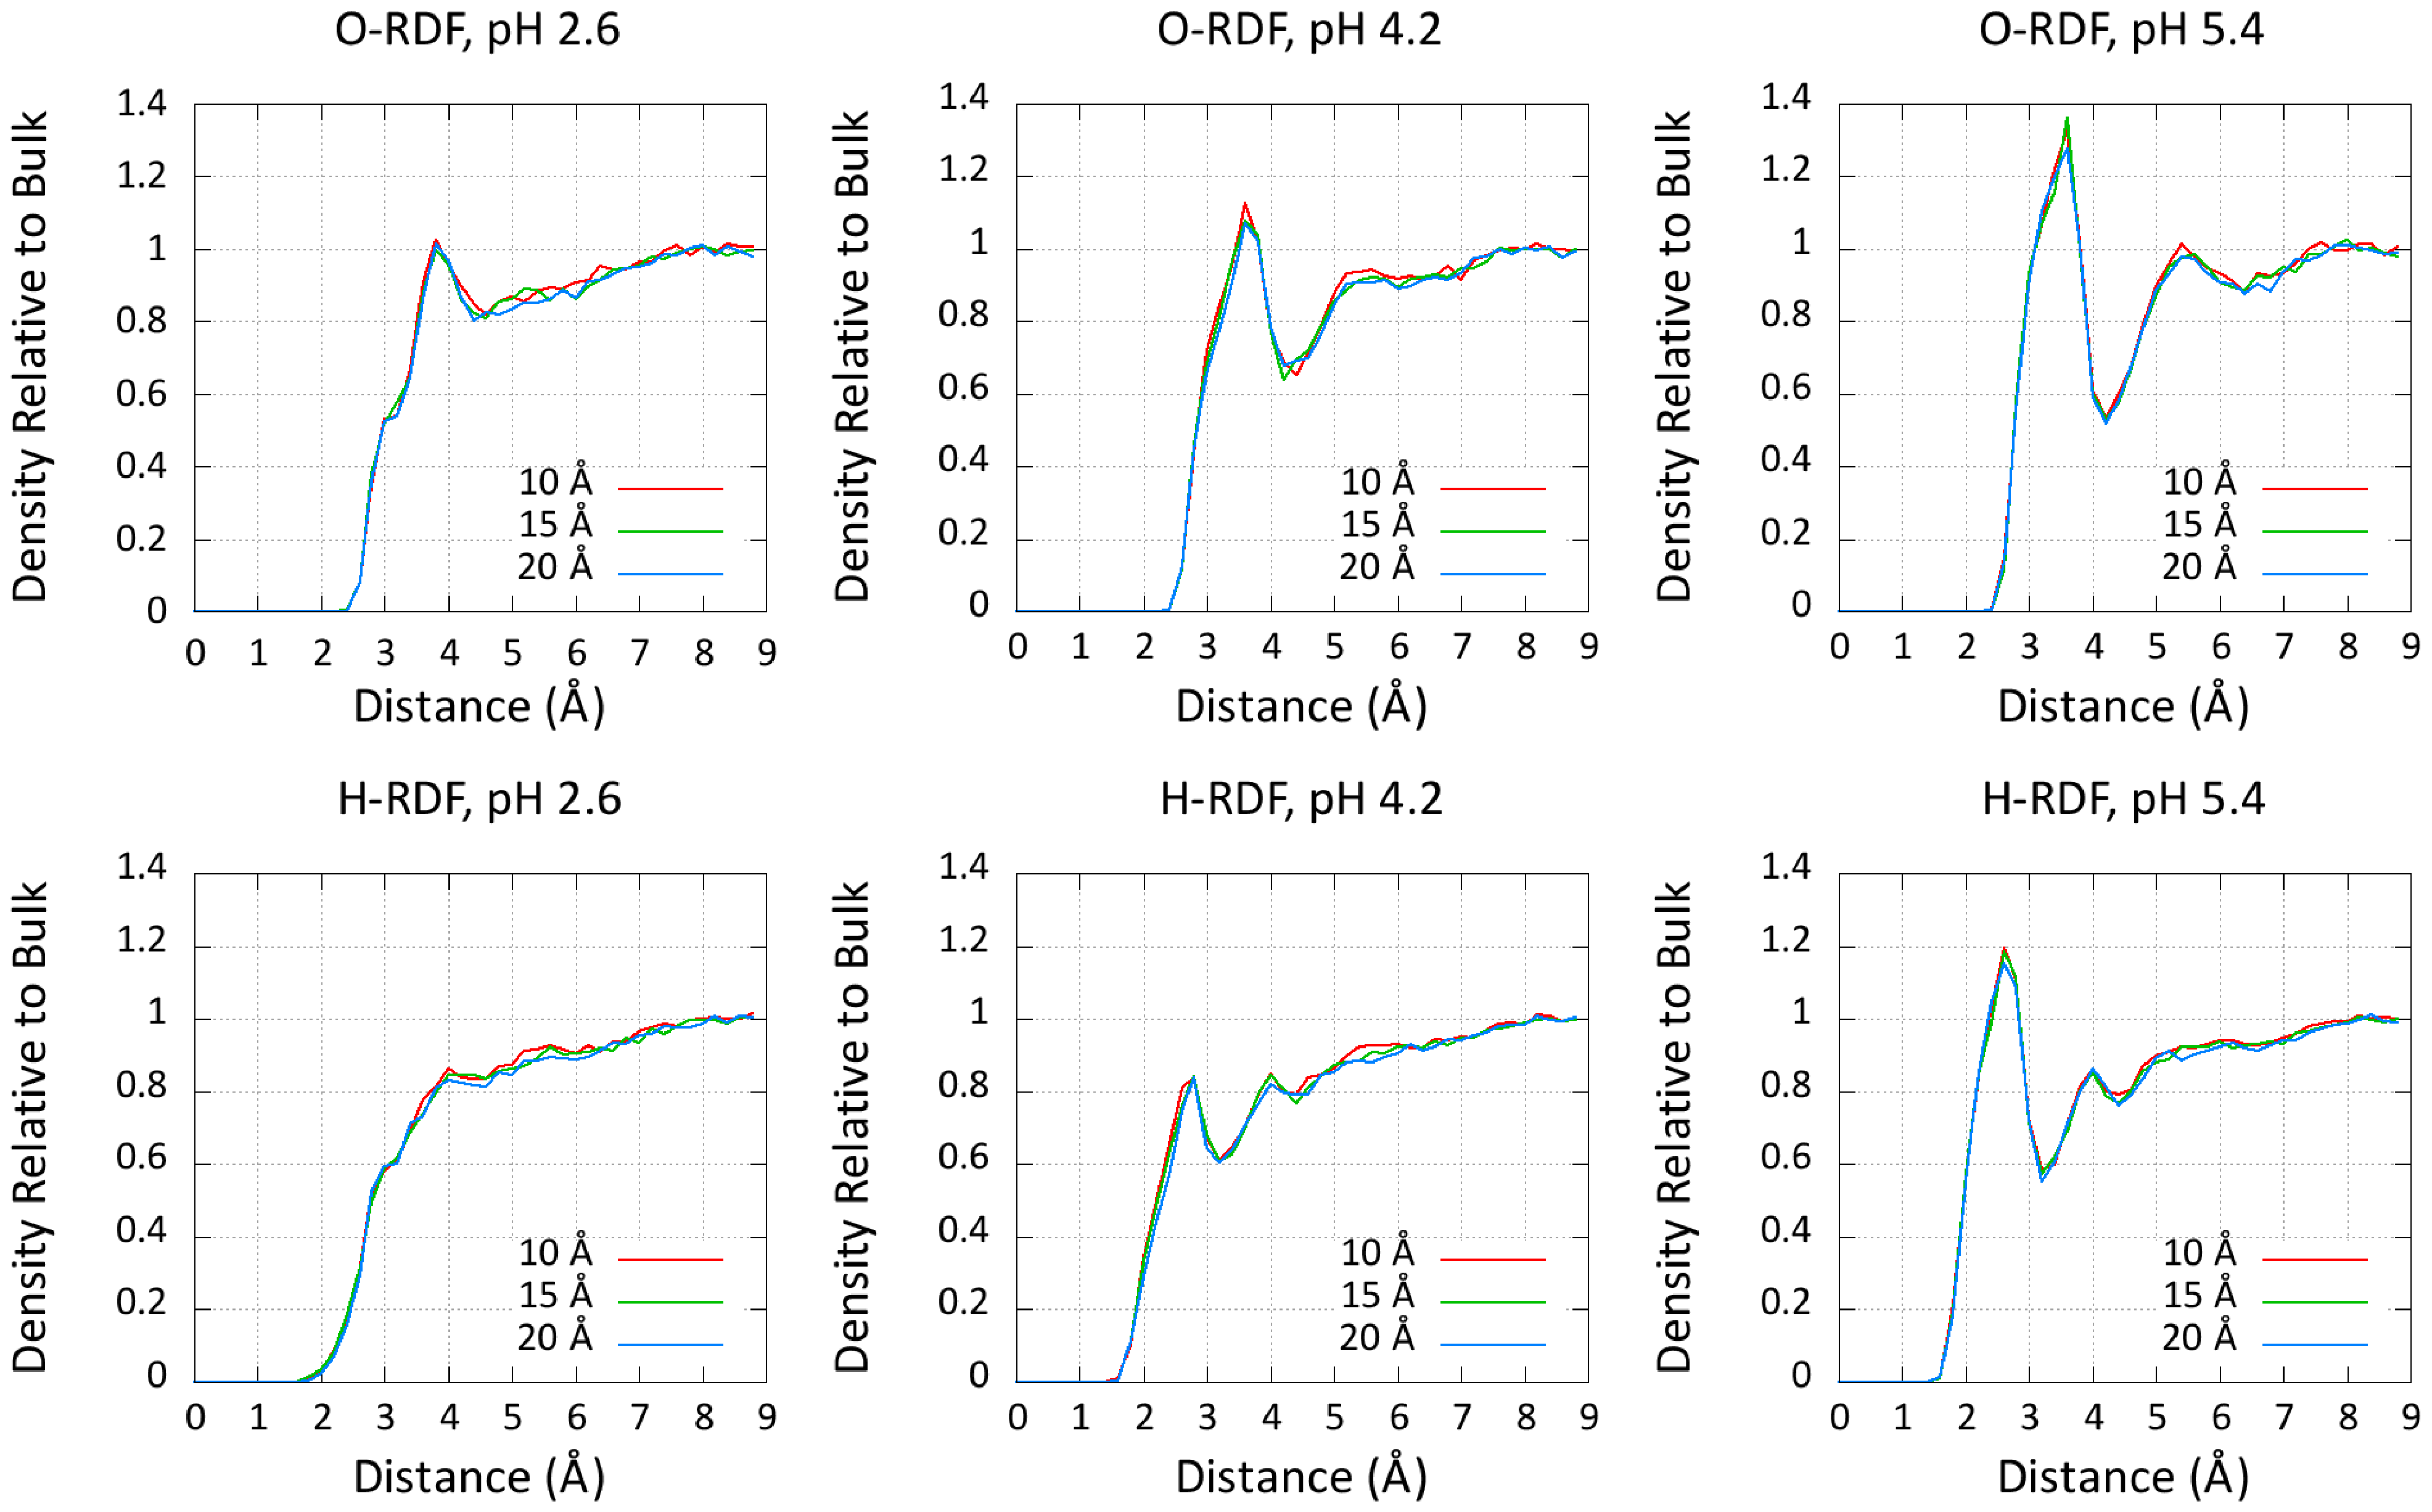
\includegraphics[width=6.5in]{model_AS4_RDF_box.eps}
   \caption{Radial distribution functions (RDFs) of solvent oxygen atoms (O) and
            hydrogen atoms (H) with different unit cell sizes. The shown
            measurements---10, 15, and 20 \text{\AA}---represent the size of the
            solvent buffer surrounding the solute. RDF plots for three different
            pHs are shown, highlighting the pH dependence of the solvent
            structure around the carboxylate of the aspartate model compound and
            its invariance to box size.}
   \label{fig4:ref_rdf}
\end{figure}

\subsection{$\tau _ {rlx}$ Effects}

An important approximation in the proposed method is that the protonation state
sampling $\rho^\prime$ from Eq. \ref{eq4:solv_sep_prob} can be replaced using an
implicit solvent model followed by relaxation MD to generate the relaxed solvent
positions and momenta. The question then becomes how long this relaxation
dynamics should be run.

To address this, 2 ns of constant protonation molecular dynamics simulations
were run on the model cysteine compound in both protonation states---protonated
and deprotonated---after the same minimization and heating protocols were used
as for the other model compound simulations. The protonation state was then
swapped for the final structures of both simulations, and MD was performed while
constraining the solute position for 20 ns, equivalent to the relaxation
dynamics protocol in our proposed method.

The optimum value for $\tau _ {rlx}$ is the time after which the energy of the
relaxation trajectory stabilizes and the simulation loses all memory of its
initial configuration. To be truly equivalent to having been chosen at random,
the final, relaxed solvent distribution must be completely uncorrelated from the
initial distribution at the time the protonation state was changed.

To probe the necessary time scales for these relaxation dynamics, the energy of
each snapshot in the relaxation trajectory is plotted alongside the
autocorrelation function of that energy in Fig. \ref{fig4:ntrelax_and_autocorr}
to clearly demonstrate the `appropriate' value of $\tau _ {rlx}$ for this model
system.

I chose the cysteine model compound for this test for two reasons. First, the
model compounds are fully solvent-exposed due to their small size, which results
in a worst-case scenario in terms of the number of water molecules that must be
reorganized during the relaxation dynamics. The optimum $\tau _ {rlx}$ value
for model compounds is expected to be an upper-bound on the values required for
larger systems. Secondly, cysteine is the smallest and simplest of the
titratable amino acids, eliminating potential complications from tautomeric
states compared to aspartate, glutamate, and histidine.

\begin{figure}
   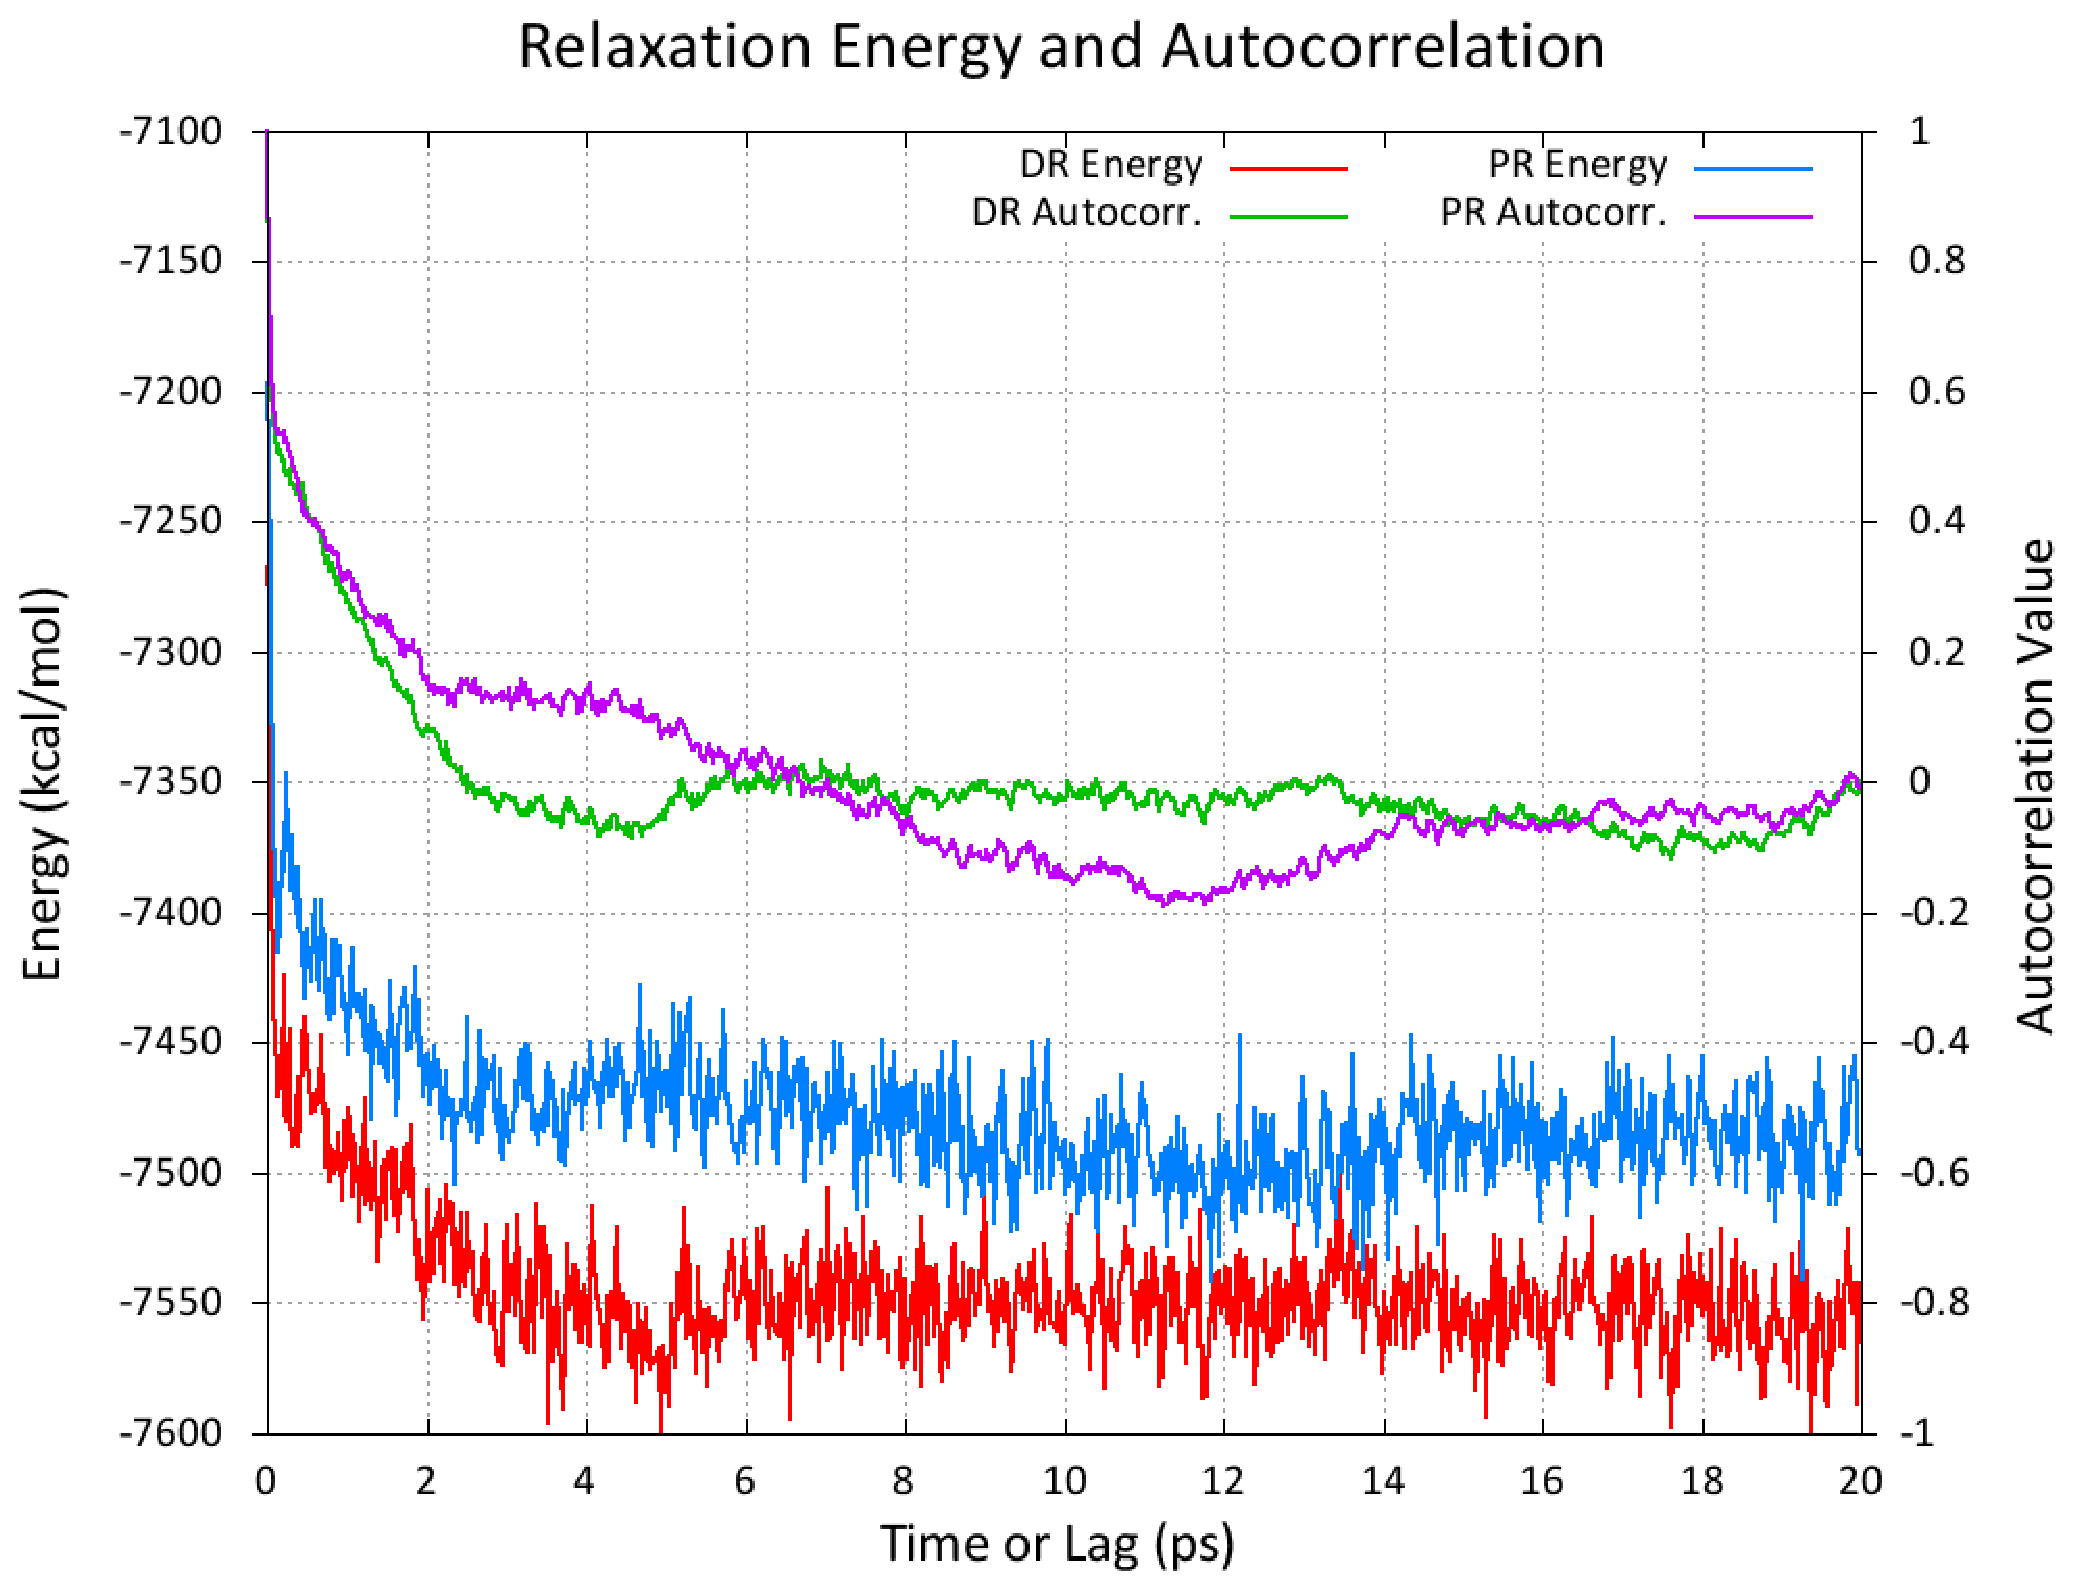
\includegraphics[width=6in]{Cys_ntrelax_energies.eps}
   \caption{The relaxation of the protonated state---starting from the
            protonated trajectory---is shown in blue with its autocorrelation
            function shown in purple. The relaxation of the deprotonated state
            from an equilibrated snapshot from the protonated ensemble is shown
            in red with its autocorrelation function shown in green. Here,
            \emph{PR} and \emph{DR} stand for \emph{Protonated-Relaxation} and
            \emph{Deprotonated-Relaxation}, respectively.}
   \label{fig4:ntrelax_and_autocorr}
\end{figure}

The relaxation energies plotted in Fig. \ref{fig4:ntrelax_and_autocorr} begin to
stabilize after 4 to 6 ps of relaxation dynamics, and the autocorrelation
function indicates that the relaxation energies are uncorrelated from the point
of the protonation state change. However, because 4 ps of MD---corresponding to
\mbox{2 000} steps of dynamics with a 2 fs time step---adds dramatically to the
cost of CpHMD simulations in explicit solvent, I explored the approximation of
using a significantly smaller value for $\tau _ {rlx}$.

Both the relaxation energies and autocorrelations drop very sharply at the start
of the relaxation dynamics, so the majority of the benefit gained by relaxing
the solvent is realized within the first few steps.

For example, the energies from the relaxation of the deprotonated structure in
the protonated state drops from -7197 kcal/mol to -7377 kcal/mol during the
first 200 fs. The average energy of the final 10 ns of that trajectory is -7490
kcal/mol. Likewise, the energies from the other relaxation dynamics drops from
-7267 kcal/mol to -7465 kcal/mol over the first 200 fs, finally settling into an
average of -7552 kcal/mol over the final 10 ns. In both cases, 70\% of the total
relaxation energy was realized during the first 200 fs of relaxation dynamics.
The autocorrelation function of the relaxation energy decays similarly, so the
assumption that the relaxed solvent distribution is uncorrelated from its
starting point is a reasonable approximation.

To validate the use of a shorter $\tau _ {rlx}$, I titrated the aspartate model
compound using pH-REMD with five different values for $\tau _ {rlx}$---10 fs, 40
fs, 100 fs, 200 fs, and 2 ps. The calculated pK\sub{a}s were 4.08 $\pm$ 0.02,
shown in Fig. \ref{fig4:pKaplot}.  Furthermore, comparing the solvent radial
distribution functions of the different solvent relaxation times (Fig.
\ref{fig4:ntrelax_rdfs}) shows little dependence of the solvent distribution on
the value of $\tau _ {rlx}$.

\begin{figure}
   \includegraphics[width=6.5in]{pKaplot.ps}
   \caption{Computed pK\sub{a}s for the Aspartate model compound using different
            relaxation times ($\tau_{rlx}$).}
   \label{fig4:pKaplot}
\end{figure}

\begin{figure}
   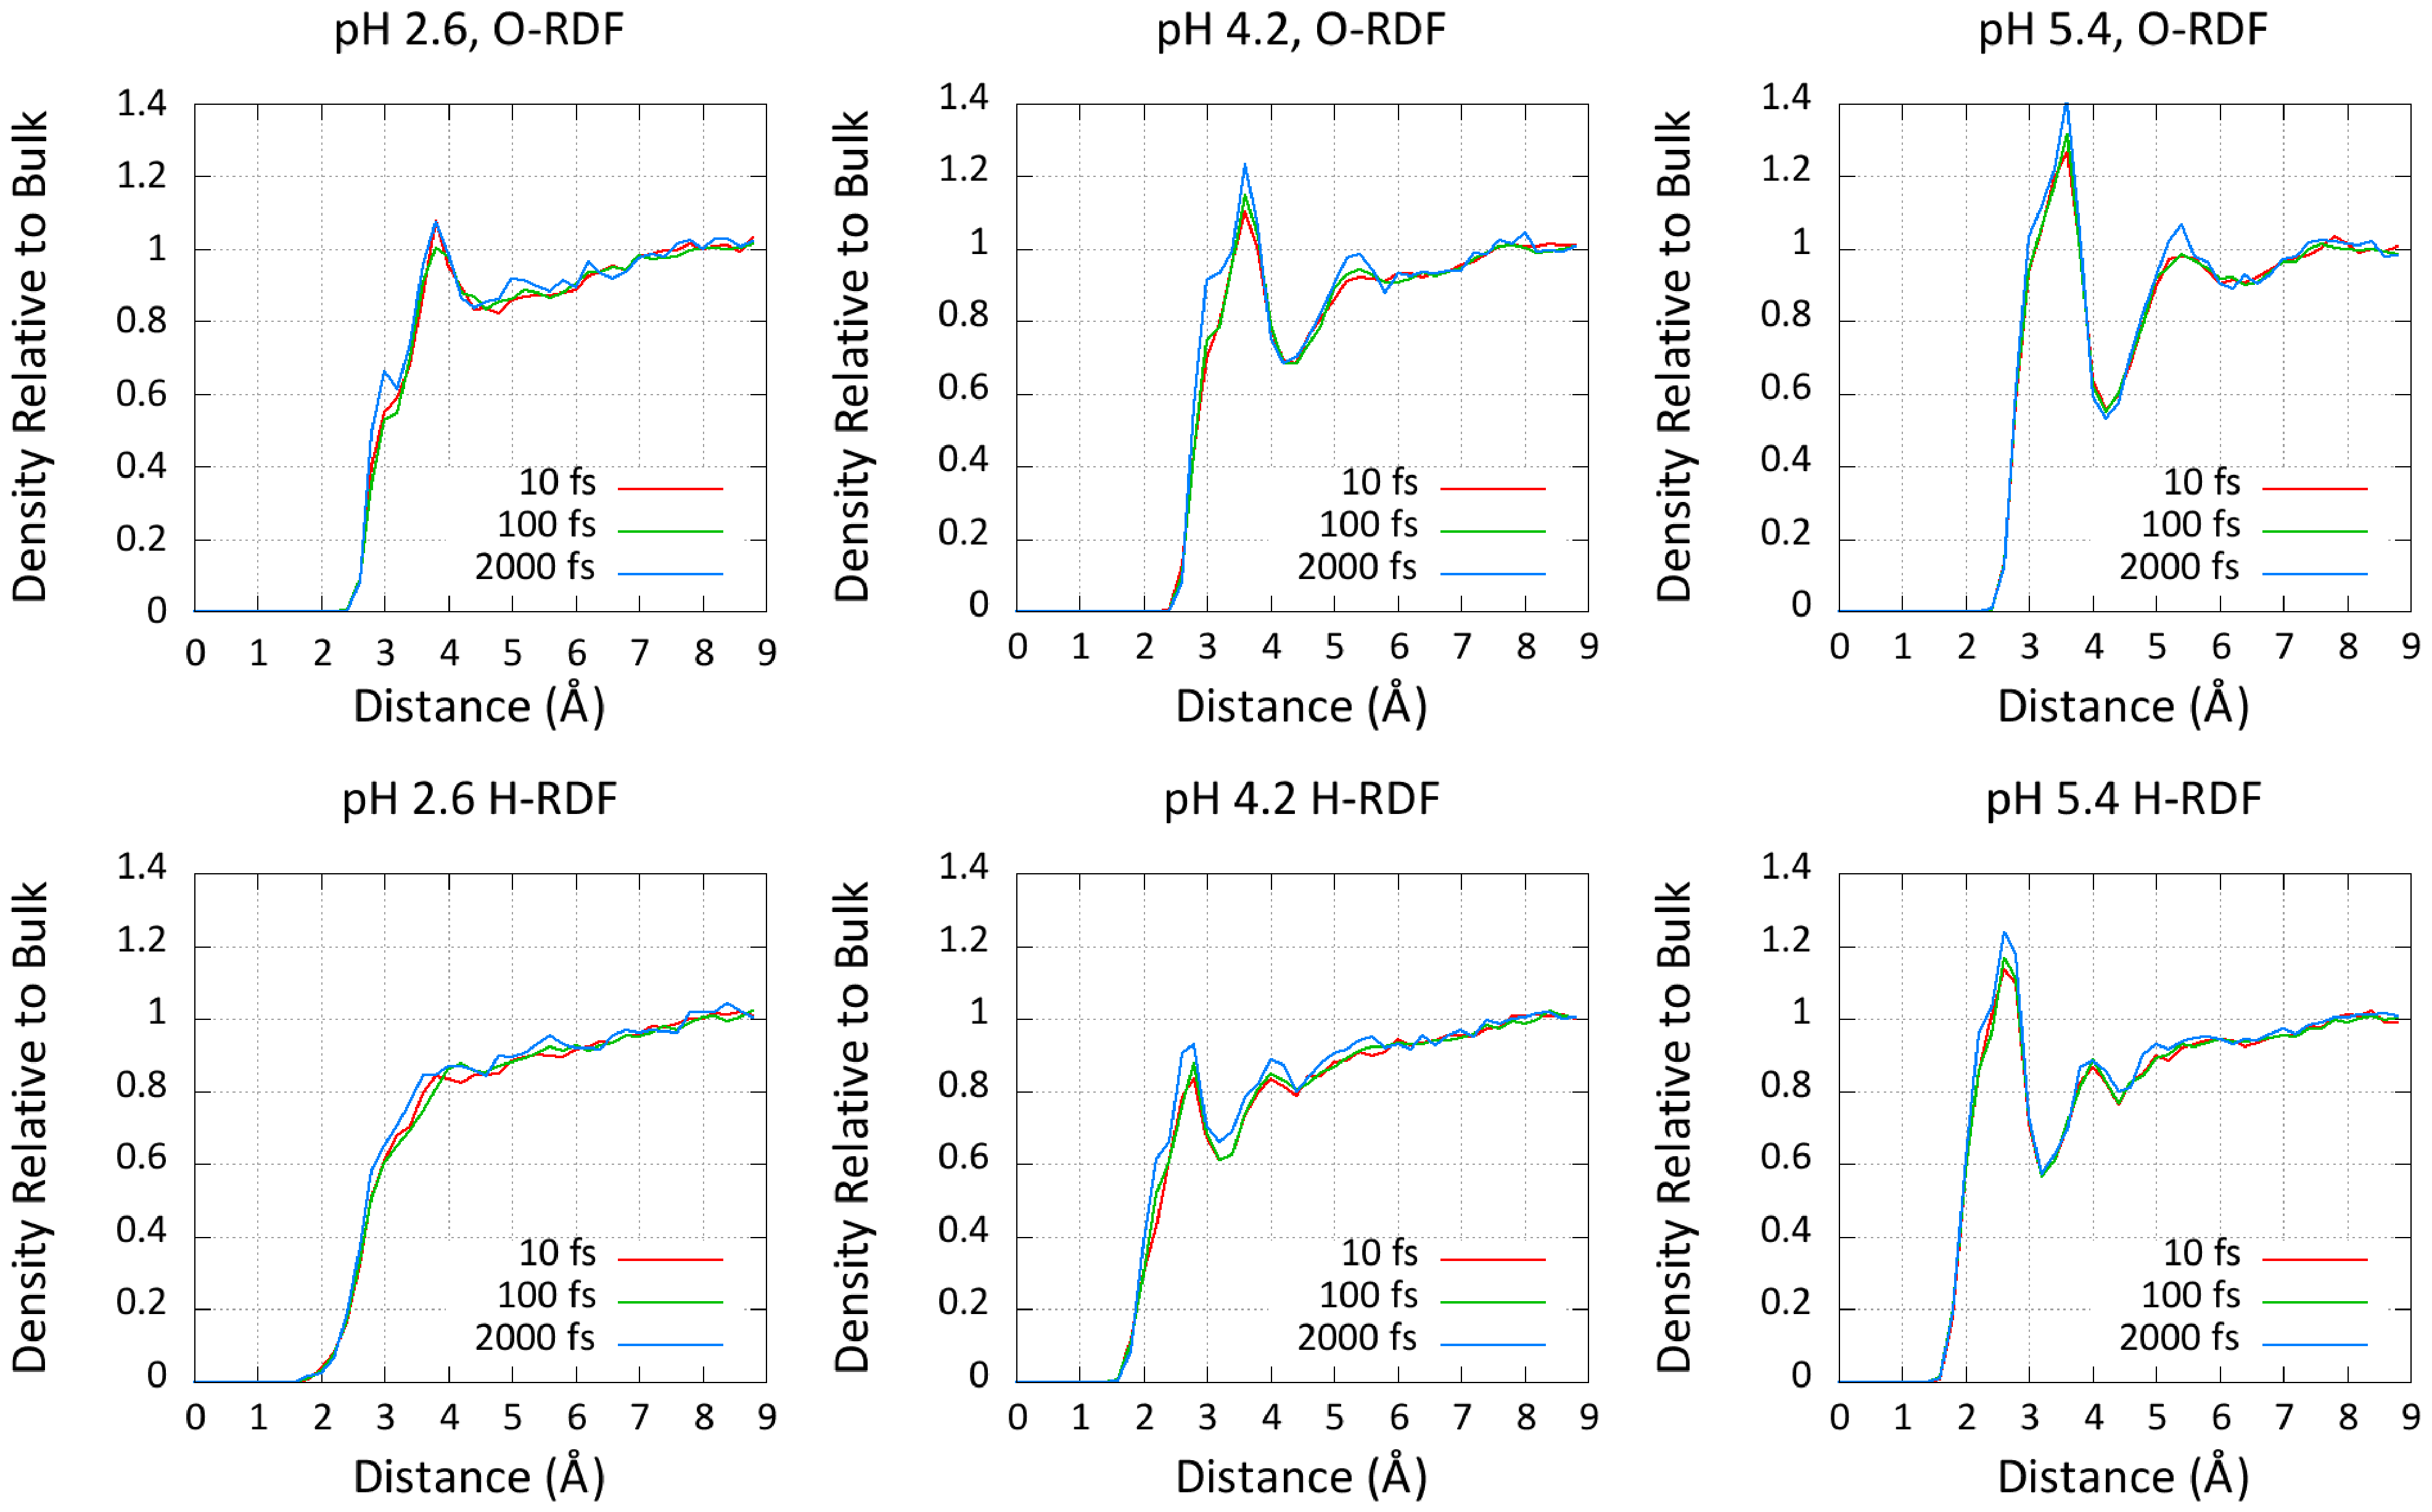
\includegraphics[width=6.5in]{ntrelax_radial_ph.eps}
   \caption{RDFs of water oxygen atoms (O) and hydrogen atoms (H) around the
            center-of-mass of the carboxylate group of the model aspartate
            molecule at different solution pHs.}
   \label{fig4:ntrelax_rdfs}
\end{figure}

\subsection{ACFCA: CpHMD vs. pH-REMD}

The small peptide chain ACFCA, described in Sec. \ref{sec4:ACFCA}, was chosen as a
test due to its small size and predictable titration behavior. The simplicity of
the system makes it an ideal test---its small size mitigates the conformational
sampling problem, and the simple titrating behavior of cysteine further
simplifies protonation state sampling. Unlike aspartate and glutamate, which
have the four defined tautomeric states defined by anti- and syn-protonation on
each of two carboxylate oxygens, and histidine which has two tautomeric states
on the imidazole, cysteine has only one protonated and one deprotonated state,
presenting fewer degrees of freedom that must be exhaustively sampled.

Each cysteine is in a slightly different micro-environment due to the different
charges of the N- and C-termini. Because Cys 2 is typically closer to the
N-terminus, it is expected to experience a negative pK\sub{a} shift with respect
to the model compound due to the electrostatic influence of the
positively-charged terminus.  Cys 4, on the other hand, is expected to
experience a pK\sub{a} shift in the opposite direction due to the electrostatic
pressure of the negatively-charged C-terminus.

I ran simulations at pH 7.1, 8.1, 8.3, 8.7, 8.9, and 9.9 to sufficiently
characterize the titration behavior of both cysteine residues around their
pK\sub{a}s. One set of replicas was run with pH-REMD while the other set was run
using CpHMD (i.e., without attempting exchanges between the replicas). The
titration curves for both sets of simulations, shown in
Fig. \ref{fig4:acfca_titration_curves}, demonstrate the importance of using
pH-REMD in constant pH simulations in explicit solvent. The pK\sub{a} of Cys 2
and Cys 4 were 8.2 and 9.4, respectively. As expected, these pK\sub{a}s
represent shifts of -0.2 pK units for Cys 2 and +0.9 pK units for Cys 4 with
respect to the model Cys compound. As a test, this compound was run using the
original CpHMD implementation in implicit solvent
\cite{Mongan_JComputChem_2004_v25_p2038} to ensure that we obtained the same
results. Because the available phase space in simulations ACFCA is so small due
to the small size of the molecule, the sampled ensembles in implicit and
explicit solvent are expected to be very similar. When run in implicit solvent,
the two cysteine residues have almost identical pK\sub{a}s to those obtained by
the simulations in explicit solvent---8.1 and 9.4, for Cys 2 and Cys 4,
respectively.

\begin{figure}
   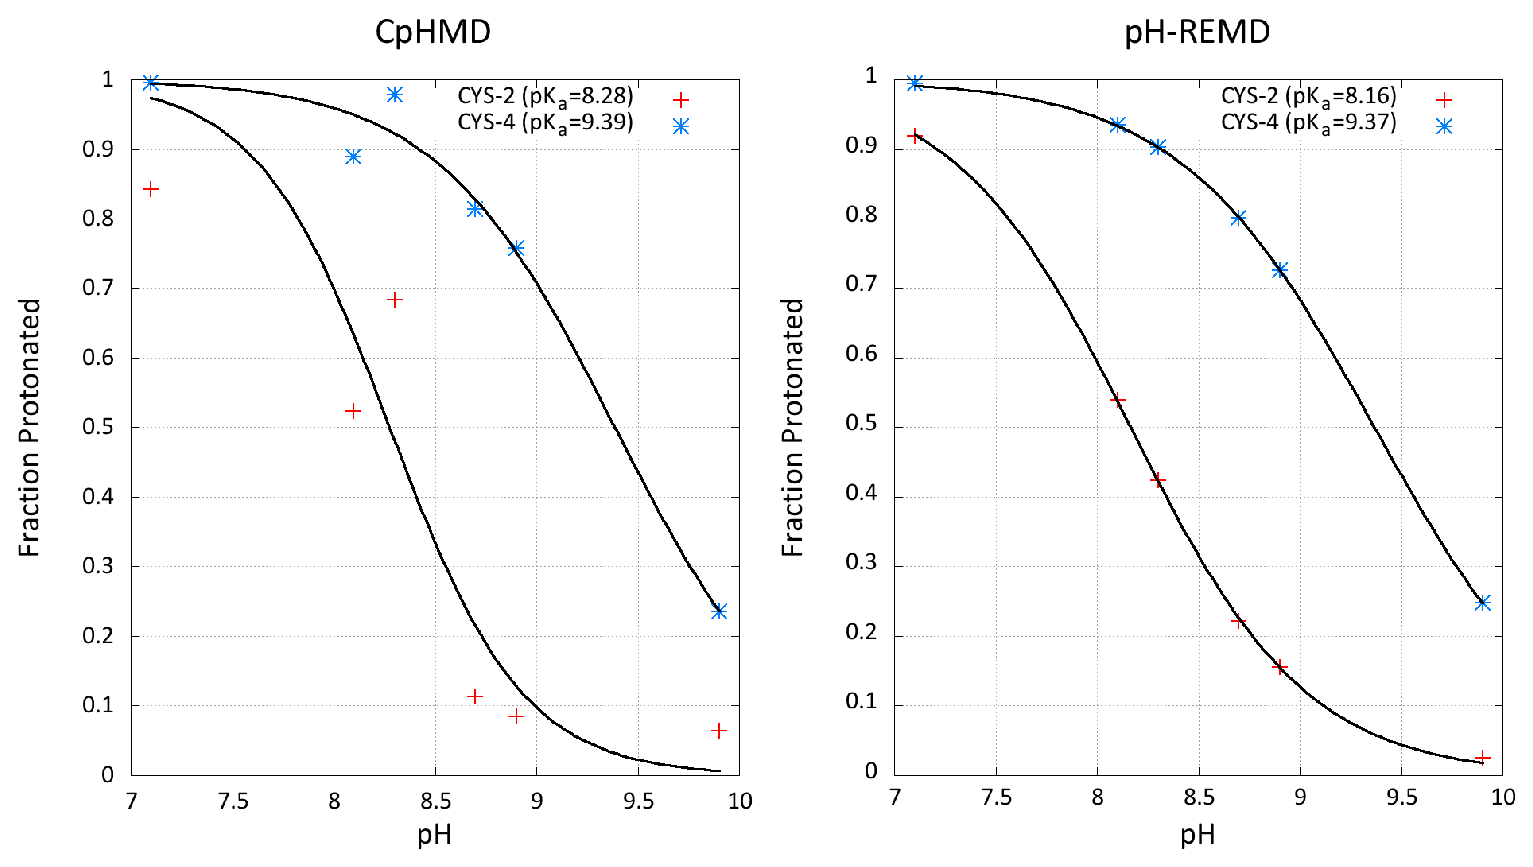
\includegraphics[width=6.5in]{ACFCA_Titration_Curves.eps}
   \caption{Titration curves of Cys 2 and Cys 4 in the \emph{ACFCA}
            pentapeptide. Results from CpHMD (no replica exchange attempts) and
            pH-REMD are shown in the plots on the left and right, respectively.}
   \label{fig4:acfca_titration_curves}
\end{figure}

Even for a simple system such as ACFCA, using pH-REMD on top of standard CpHMD
simulations results in a drastic improvement in titration curve fit---a result
of improved protonation state sampling. The residual sum of squares (RSS), a
quantity that measures how well an equation fits a data set whose equation is
shown in \ref{eq3:fit_quality}, shows drastic improvement using pH-REMD. The RSS
for Cys 2 and Cys 4 using CpHMD was $9 \times 10 ^ {-2}$ and $7 \times 10 ^
{-3}$, respectively. For the pH-REMD simulations, on the other hand, the RSS was
reduced by several orders of magnitude to $7 \times 10 ^ {-5}$ and $9 \times 10
^ {-6}$ for Cys 2 and Cys 4, respectively.

\subsection{Hen Egg White Lysozyme}

HEWL is a common benchmark for pK\sub{a} calculations because it has been
studied extensively both experimentally
\cite{Takahashi_Biopolymers_1992_v32_p897, Bartik_BiophysJ_1994_v66_p1180,
Webb_Proteins_2011_v79_p685} and theoretically,
\cite{Mongan_JComputChem_2004_v25_p2038, Demchuk_JPhysChem_1996_v100_p17373,
Williams_JChemTheoryComput_2010_v6_p560, Machuqueiro_Proteins_2008_v72_p289,
Swails_JChemTheoryComput_2012_v8_p4393, Wallace_JChemTheoryComput_2011_v7_p2617}
and it has a large number of titratable residues---some with a marked pK\sub{a}
shift compared to the isolated model compound.

The 1AKI and 4LYT crystal structures were prepared initially without any ions,
resulting in unit cells with a net charge of +9 electrons when the carboxylate
residues are negatively charged and the histidine residue is positively charged.
The calculated pK\sub{a} for all 10 residues that titrate in the acidic range
are summarized in Table \ref{tbl4:hewl_noions_pkas} for both starting
structures.

\begin{table}
   \caption{Calculated pK\sub{a}s for acid-range titratable residues in HEWL
            using the proposed method for both starting structures---PDBs 1AKI
            and 4LYT---without ions. The root mean square error (RMSE) and mean
            unsigned error (MUE) with respect to the experimental values are
            shown in the last two rows.  Experimental values are taken from
            \citeauthor{Webb_Proteins_2011_v79_p685}
            \cite{Webb_Proteins_2011_v79_p685}}
   \begin{tabular}{cccc}
      Residue & PDB 1AKI & PDB 4LYT & Experiment
                                 \cite{Webb_Proteins_2011_v79_p685} \\
      \hline
      Glu 7 & 1.6 & 1.8 & 2.6 \\
      His 15 & 7.1 & 6.5 & 5.5 \\
      Asp 18 & 1.8 & 1.8 & 2.8 \\
      Glu 35 & 5.0 & 4.9 & 6.1 \\
      Asp 48 & -0.2 & -0.3 & 1.4 \\
      Asp 52 & -0.3 & -1.2 & 3.6 \\
      Asp 66 & -1.8 & -1.0 & 1.2 \\
      Asp 87 & 0.5 & 0.5 & 2.2 \\
      Asp 101 & 3.7 & 3.8 & 4.5 \\
      Asp 119 & 0.0 & 0.3 & 3.5 \\
      \hline
      \hline
      \textbf{RMSE} & \textbf{2.19} & \textbf{2.20} & --- \\
      \textbf{MUE} & \textbf{1.91} & \textbf{1.83} & --- \\
      \hline
   \end{tabular}
   \label{tbl4:hewl_noions_pkas}
\end{table}

The pK\sub{a}s predicted here agree worse than our results presented in Ref.
\citenum{Swails_JChemTheoryComput_2012_v8_p4393}, due mainly to the poor
treatment of aspartate residues 48, 52, 66, and 119. The disparity between the
implicit and explicit solvent results probably stems from the enhanced
conformational sampling attainable with implicit solvent simulations. Dynamical
events occur much slower in explicit solvent simulations due to the friction and
viscosity of the solvent. However, the conformations sampled in implicit solvent
are frequently artifacts of the inaccuracies in the underlying solvent model
\cite{Zhou_Proteins_2003_v53_p148, Geney_JChemTheoryComput_2006_v2_p115} that
may hinder the performance of the CpHMD simulations.
\cite{Machuqueiro_Proteins_2011_v79_p3437}

The difference in the conformational sampling ability of the proposed method and
the original, implicit solvent-based method is pronounced enough that a simple
comparison of the root mean squared deviation (RMSD) is a sufficient
illustration. The RMSD of the trajectories in the current study (Fig.
\ref{fig4:hewl_rmsd}) is 2 to 3 times smaller than the RMSDs shown in Fig.
\ref{fig3:RMSD_bin} from Ch. \ref{ch3}, despite the extra 4 ns of production MD
performed for each replica in explicit solvent. Furthermore, the dynamics
displays none of the regions of flexibility noted in implicit solvent that were
correlated with the improved titration of aspartate 66.
\cite{Swails_JChemTheoryComput_2012_v8_p4393}

\begin{figure}
   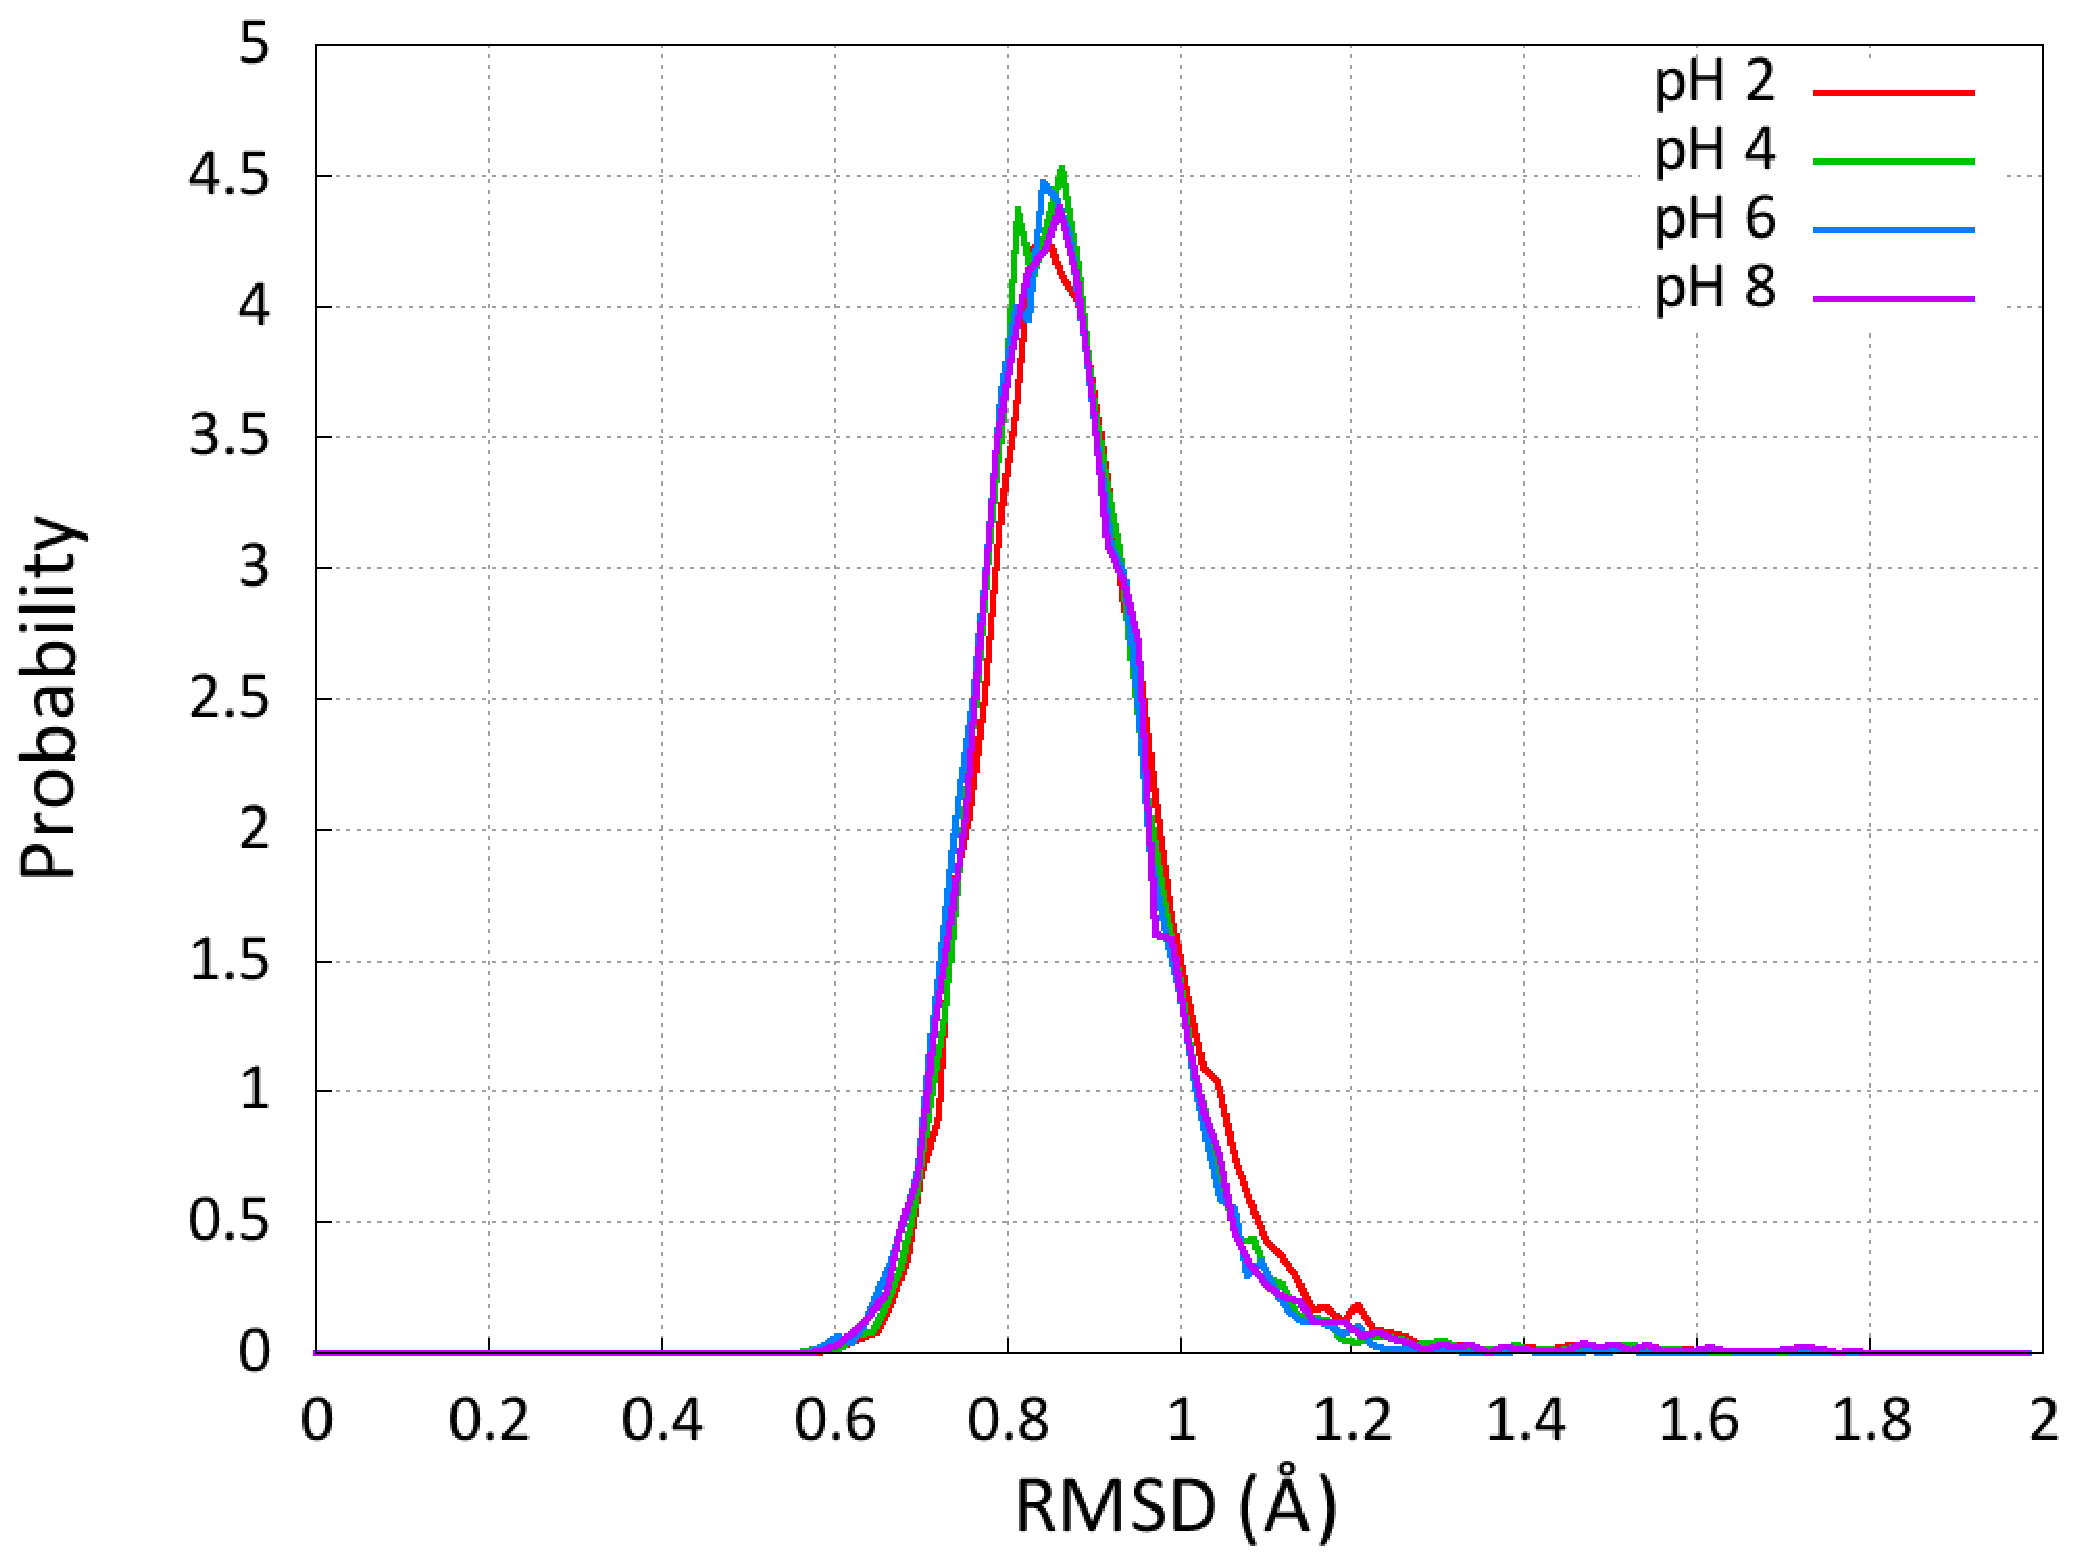
\includegraphics[width=6.5in]{1AKI_RMSDs.eps}
   \caption{RMSD plots over 20 ns of pH-REMD simulation for HEWL at pH 2, 4, 6
            and 8 with respect to the starting crystal structure 1AKI. The
            distributions are very similar for the starting structure 4LYT as
            well.}
   \label{fig4:hewl_rmsd}
\end{figure}

\subsubsection*{Ions}

When all aspartate and glutamate residues are deprotonated and the histidine is
protonated at both the $\delta$ and $\epsilon$ positions, HEWL has a net charge
of +9 electrons. Even though the PME implementation in Amber applies a net
neutralizing plasma for such systems, the lack of counterions in the unit cell
may lead to unusual behavior by any of the 30 charged residues in the system.

Therefore, I added 21 ions---15 chloride and 6 sodium---to add ionic strength
and to provide the ions necessary to neutralize the initial unit cell. Like the
effects of the unit cell size and $\tau _ {rlx}$ value, ions will only affect
the calculated pK\sub{a}s by modifying the sampled conformations since the
protonation state changes are performed using implicit solvent.

The predicted pK\sub{a}s, shown in Table \ref{tbl4:hewl_ions_pkas}, show a
marked improvement for several residues whose calculated pK\sub{a} was too low
without ions.  The simulations with explicit ions did not exhibit heightened
sampling of large-scale conformational changes---the RMSD plots of these
simulations are shown in Fig. \ref{fig4:hewl_ions_rmsd}---but is rather a result
of changes to the microenvironment around the relevant titratable residues
significant enough to effect a noticeable change to the titrating behavior.

The residue that experienced the largest pK\sub{a} shift as a result of the
added ions was Asp 66. As I observed in our previous work, Asp 66 is surrounded
by proton donors, such as the Arg 68 and the hydroxyl groups of Thr 69 and Ser
60. \cite{Swails_JChemTheoryComput_2012_v8_p4393} The arginine residue, carrying
a net positive charge, is the strongest driving force favoring the deprotonated
state. To compare how Arg 68 may affect Asp 66 differently when ions are
present, I show in Fig. \ref{fig4:hewl_asparg_dist} that the distribution of
Asp 66--Arg 68 distances is shifted to larger values when ions are present.
Because Arg 68 can occasionally interact with chloride ions in the bulk solvent
when they are present instead of Asp 66, Asp 66 is more likely to accept
proposed protonation moves when these ions are present.

It is surprising that the presence of ions can have such a large impact on
predicted pK\sub{a}s without inducing global conformation changes. That the ions
are not included in the GB-based, protonation state changes only increases the
peculiarity of this result. Explicit ions can modify the local environment
around titratable residues enough to induce large pK\sub{a} shifts, making them
important to include in the proposed method.

\begin{table}
   \caption{Calculated pK\sub{a}s for acid-range titratable residues in HEWL
            using the proposed method for both starting structures---PDBs 1AKI
            and 4LYT---with 21 added ions. The root mean square error (RMSE) and
            mean unsigned error (MUE) with respect to the experimental values
            are shown in the last two rows.  Experimental values are taken from
            \citeauthor{Webb_Proteins_2011_v79_p685}
            \cite{Webb_Proteins_2011_v79_p685}}
   \begin{tabular}{cccc}
      Residue & PDB 1AKI & PDB 4LYT & Experiment
                                 \cite{Webb_Proteins_2011_v79_p685} \\
      \hline
      Glu 7 & 1.9 & 1.8 & 2.6 \\
      His 15 & 6.4 & 6.3 & 5.5 \\
      Asp 18 & 1.9 & 1.7 & 2.8 \\
      Glu 35 & 4.6 & 4.9 & 6.1 \\
      Asp 48 & -1.4 & 0.8 & 1.4 \\
      Asp 52 & 0.5 & 0.1 & 3.6 \\
      Asp 66 & 0.2 & -0.4 & 1.2 \\
      Asp 87 & 0.4 & 0.5 & 2.2 \\
      Asp 101 & 3.5 & 3.5 & 4.5 \\
      Asp 119 & 0.6 & -0.3 & 3.5 \\
      \hline
      \hline
      \textbf{RMSE} & \textbf{1.89} & \textbf{1.91} & --- \\
      \textbf{MUE} & \textbf{1.68} & \textbf{1.56} & --- \\
      \hline
   \end{tabular}
   \label{tbl4:hewl_ions_pkas}
\end{table}

\begin{figure}
   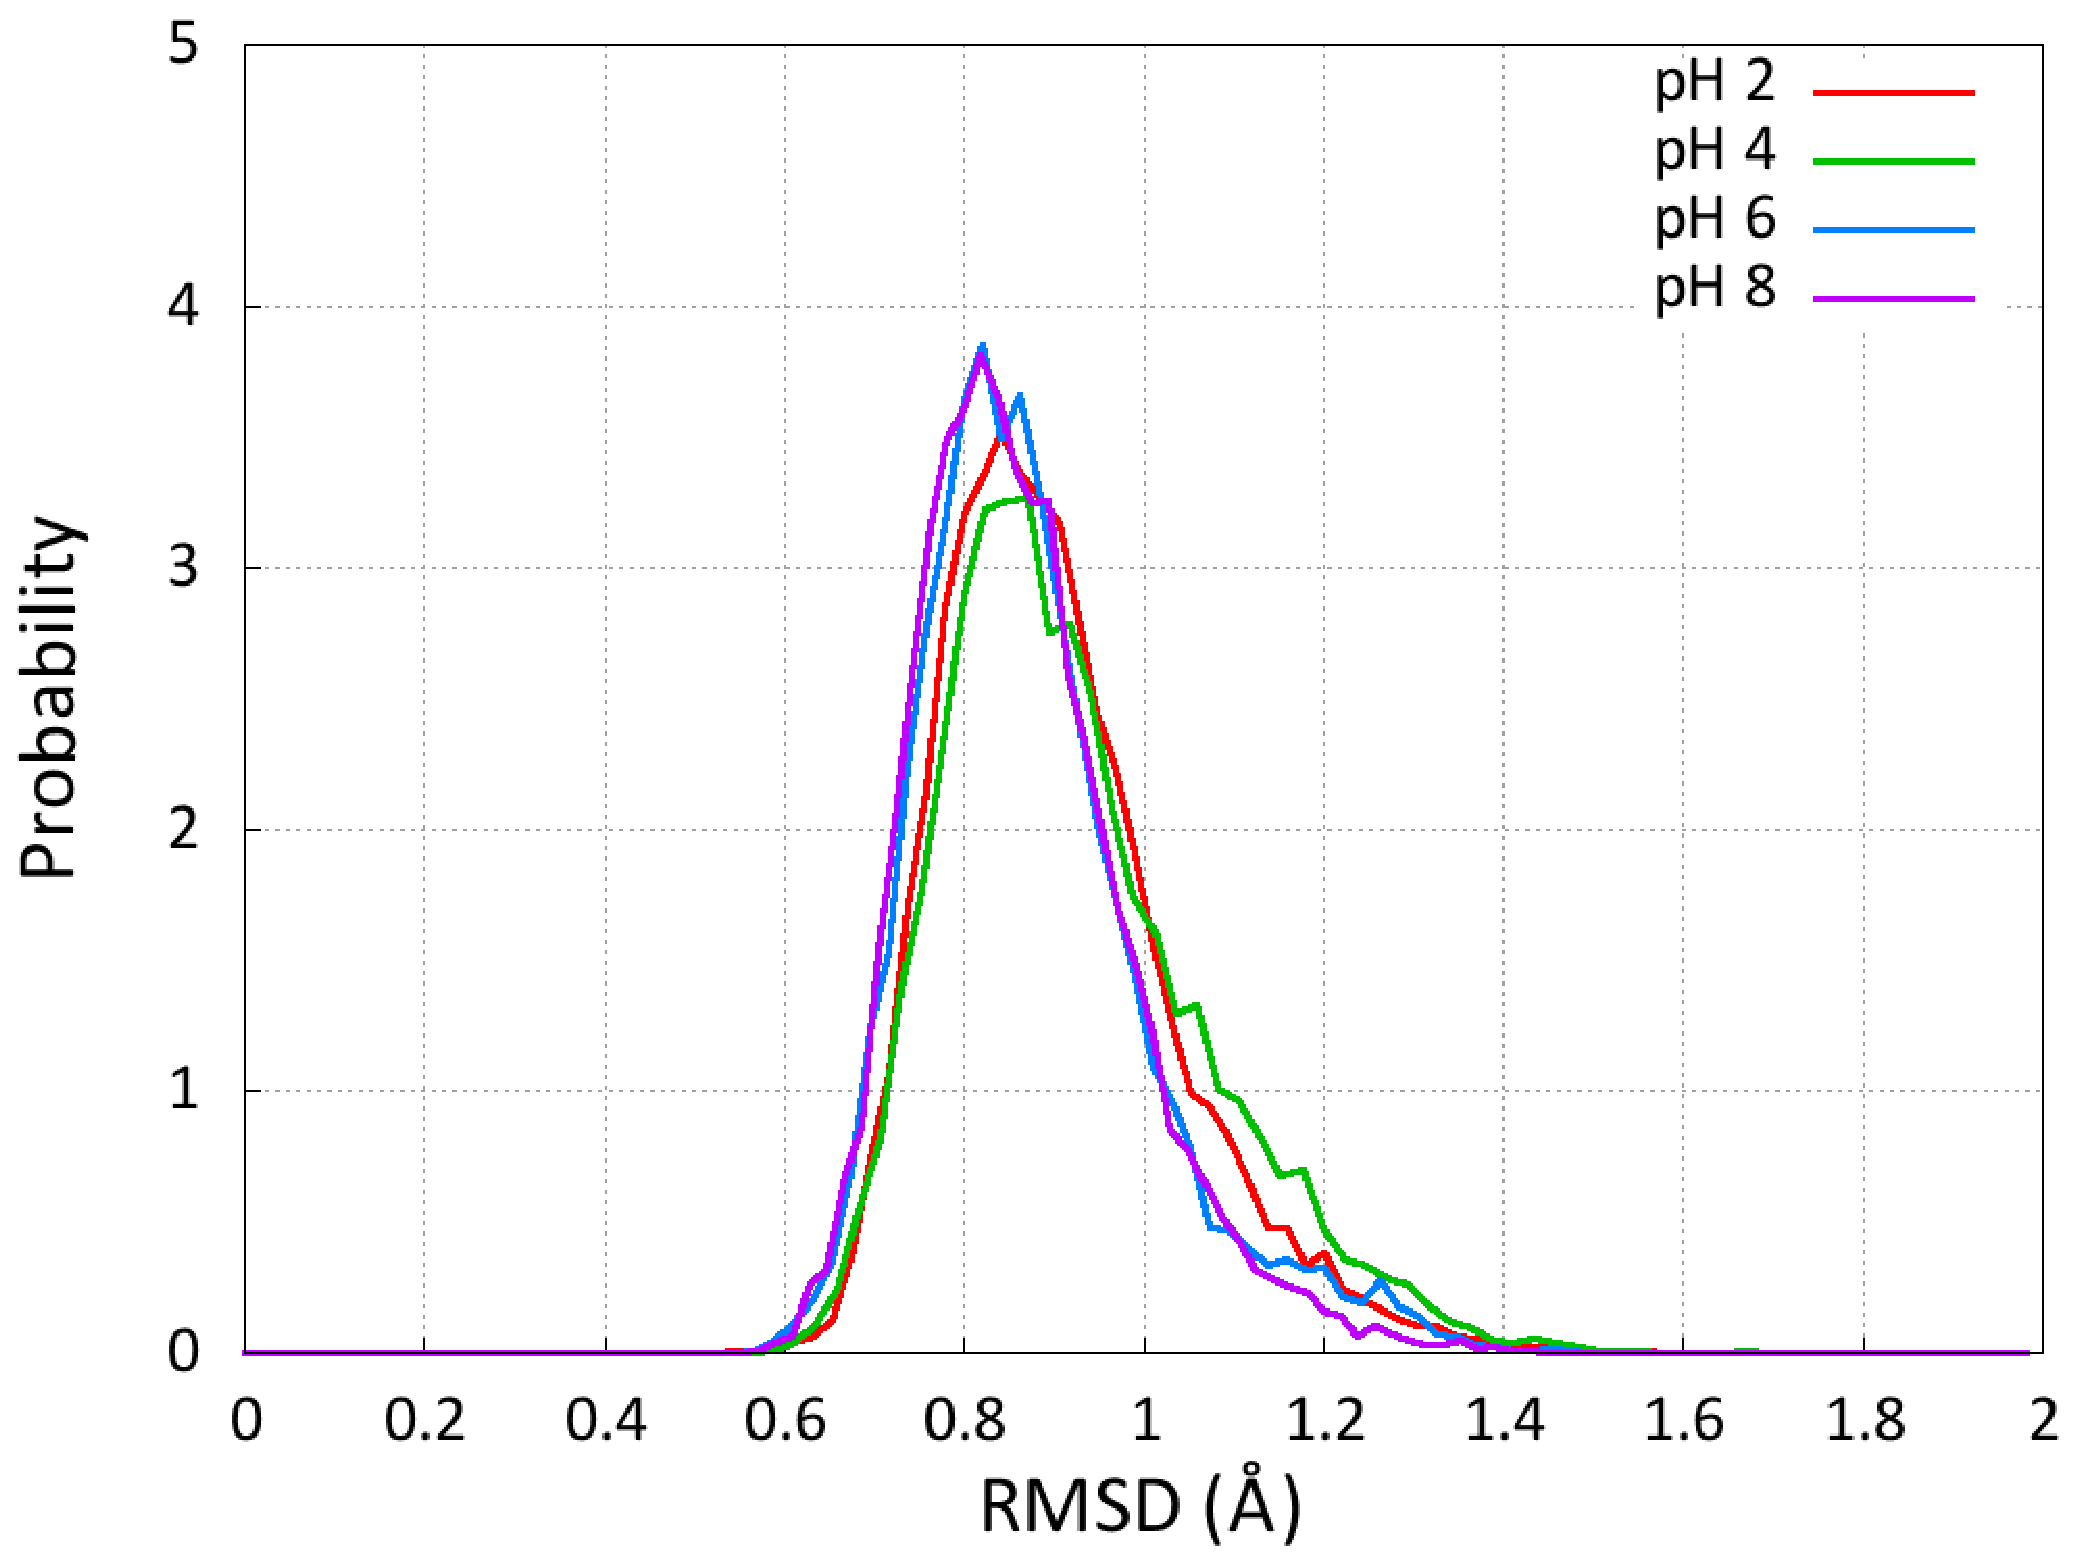
\includegraphics[width=6.5in]{1AKI_RMSDs_wions.eps}
   \caption{RMSD plots over 20 ns of pH-REMD simulation with explicit
            counterions for HEWL at pH 2, 4, 6 and 8 with respect to the
            starting crystal structure 1AKI.}
   \label{fig4:hewl_ions_rmsd}
\end{figure}

\begin{figure}
   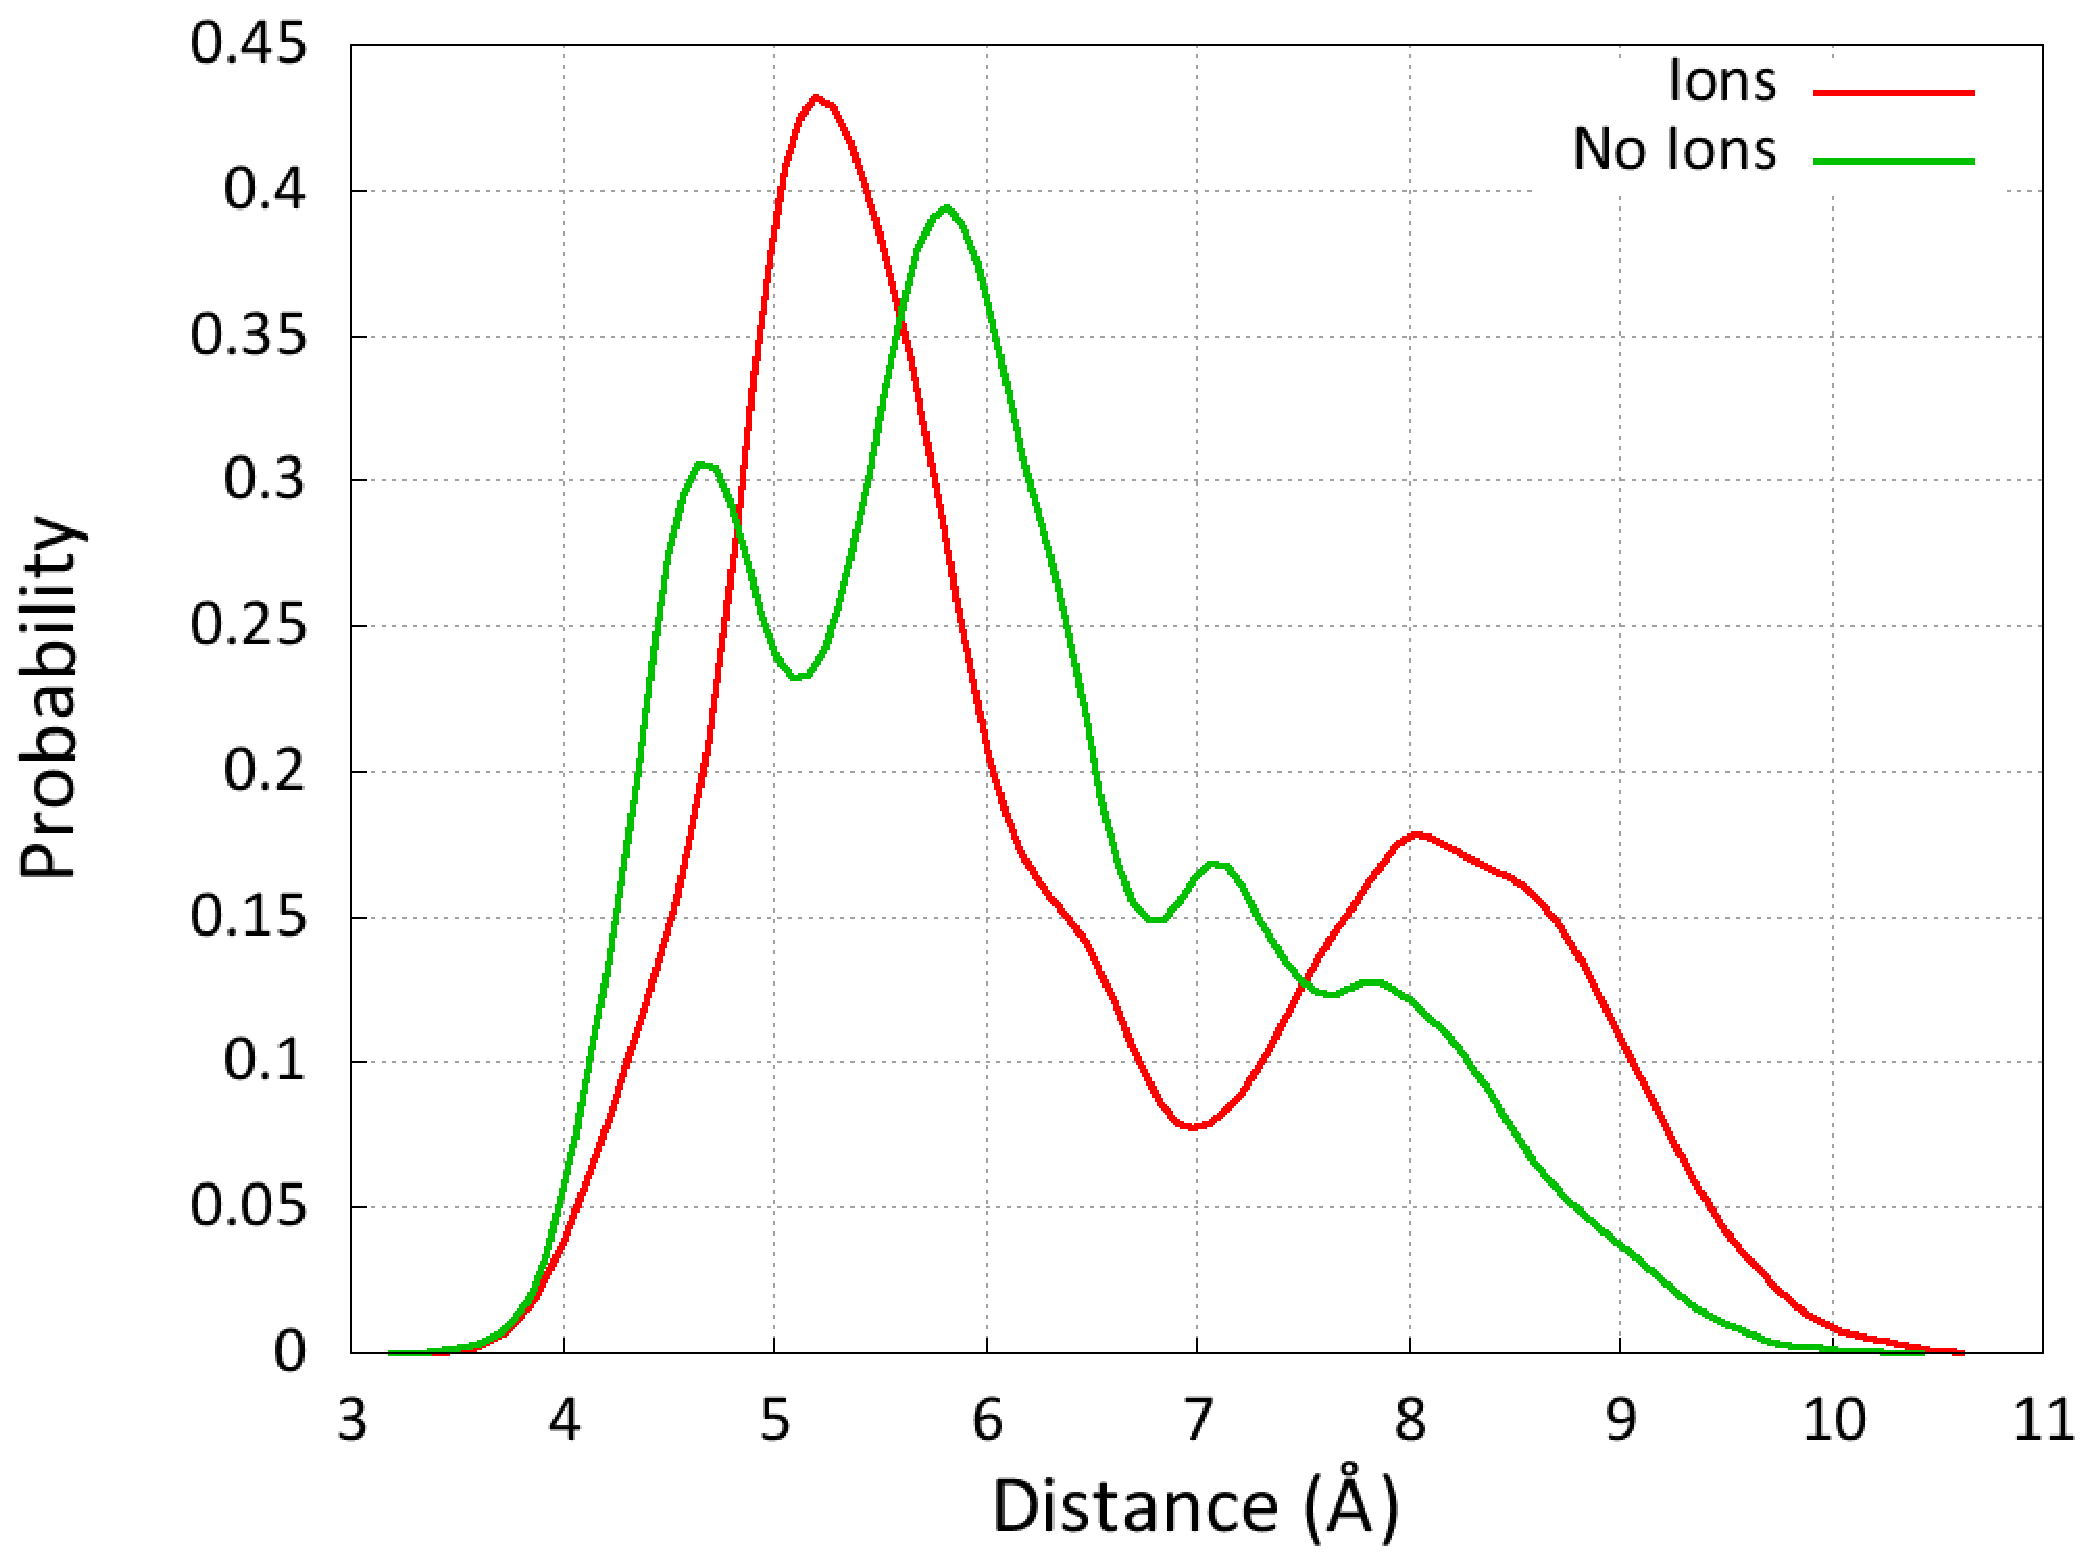
\includegraphics[width=6.5in]{HEWL_AspArg_Dist_Ion_Comparison.eps}
   \caption{Distance distribution functions calculated from HEWL simulations
            begun with crystal structure 1AKI for all snapshots in the ensemble
            at pH 1.0. The probability distributions were calculated using
            \mbox{10 000} snapshots and smoothed using a gaussian kernel density
            estimate with a bandwidth of 0.1}
   \label{fig4:hewl_asparg_dist}
\end{figure}

\subsection{Ribonuclease A}

Like HEWL, RNase A is a common benchmark for constant pH studies due to its
large number of titrating residues. Furthermore, the currently proposed
mechanism requires one catalytic histidine to be a proton donor (general acid)
and another to be a proton acceptor (general base)---His 119 and His 12,
respectively. Because a specific combination of protonation states are necessary
for catalysis, the proposed method is a useful tool for probing the
pH-dependence of RNase A.

The predicted pK\sub{a}s for RNase A in an acidic-range titration---summarized
in Table \ref{tbl4:rnase_a_pkas}---are in better agreement with experiment than
those from HEWL. This is expected, however, since the average magnitude of the
pK\sub{a} shifts with respect to the model compounds is smaller in RNase A.

\begin{table}
   \caption{Calculated pK\sub{a}s for RNase A using simulations begun from
            crystal structures 1KF5 and 7RSA. Experimental values shown are
            taken from Ref. \citenum{Baker_ArchBiochemBiophys_1996_v327_p189}.
            Root mean squared error (RMSE) and mean unsigned error (MUE) does
            not include His 48 for the 1KF5 structure or Asp 14 for the 7RSA
            structure.}
   \begin{tabular}{cccc}
      Residue & PDB 1KF5 & PDB 7RSA & Experiment
                               \cite{Baker_ArchBiochemBiophys_1996_v327_p189} \\
      \hline
      Glu 2 & -5.7 & -0.2 & 2.5 \\
      Glu 9 & 3.6 & 3.6 & 3.9 \\
      His 12 & 6.1 & 5.8 & 6.0 \\
      Asp 14 & -1.2 & -8.8 & 1.8 \\
      Asp 38 & 2.1 & 2.3 & 2.1 \\
      His 48 & $Inf$ & 5.8 & 6.1 \\
      Glu 49 & 3.4 & 3.3 & 4.3 \\
      Asp 53 & 3.6 & 3.7 & 3.7 \\
      Asp 83 & 1.6 & 1.8 & 3.3 \\
      Glu 86 & 4.3 & 4.3 & 4.0 \\
      His 105 & 7.3 & 7.8 & 6.5 \\
      Glu 111 & 3.6 & 3.4 & 3.8 \\
      His 119 & 6.0 & 6.0 & 6.5 \\
      Asp 121 & 0.6 & -0.8 & 3.0 \\
      \hline
      \hline
      \textbf{RMSE}* & \textbf{1.83} & \textbf{2.20} & --- \\
      \textbf{MUE}* & \textbf{1.18} & \textbf{1.26} & --- \\
      \hline
   \end{tabular}
   \label{tbl4:rnase_a_pkas}
\end{table}

While most of the residues have a calculated pK\sub{a} close to the experimental
value, several are trapped in environments that resist changing their
protonation state across the entire range of simulated pHs. Glu 2 is adjacent to
the N-terminal lysine residue with a +2 charge and interacts closely with the
positively-charged lysine 7 and arginine 10 residues much of the time, pushing
the predicted pK\sub{a} very low. If the time scale of the simulation is
insufficient to escape this local conformational basin, the predicted pK\sub{a}
of Glu 2 will be unphysically low, as seen in Table \ref{tbl4:rnase_a_pkas} for
the 1KF5 structure.

Similar traps are seen around Asp 14, which is surrounded by hydrogen bond
donors. The His 48 residue, on the other hand, interacts closely with numerous
backbone carbonyl atoms in a configuration that resists deprotonating either
N$^\delta$ or N$^\epsilon$ in the 1KF5 starting structure.

Like with the HEWL simulations, I ran a second set of 20 ns simulations in
which I added 14 chloride and 6 sodium ions to generate a net ion concentration
around 0.18 M. More chloride was added because the net charge of the initial
protonation states was +8 electrons. The predicted pK\sub{a}s for the
simulations with explicit counterions resulted in marked improvement in most
titratable residues that proved problematic in the simulations without the ions,
following the trend seen in the HEWL calculations. The full summary of
calculated pK\sub{a}s is shown in Table \ref{tbl4:rnase_a_ions_pkas}.
\begin{table}
   \caption{Calculated pK\sub{a}s for RNase A simulations run with explicit
            counterions present. All calculated pK\sub{a}s are included in the
            calculated root mean squared error (RMSE) and mean unsigned error
            (MUE).}
   \begin{tabular}{cccc}
      Residue & PDB 1KF5 & PDB 7RSA & Experiment
                               \cite{Baker_ArchBiochemBiophys_1996_v327_p189} \\
      \hline
      Glu 2 & 0.6 & -1.8 & 2.5 \\
      Glu 9 & 3.7 & 3.6 & 3.9 \\
      His 12 & 6.2 & 6.9 & 6.0 \\
      Asp 14 & -1.4 & -0.3 & 1.8 \\
      Asp 38 & 1.8 & 2.3 & 2.1 \\
      His 48 & 7.9 & 6.7 & 6.1 \\
      Glu 49 & 4.2 & 5.2 & 4.3 \\
      Asp 53 & 3.3 & 2.5 & 3.7 \\
      Asp 83 & 1.5 & 1.3 & 3.3 \\
      Glu 86 & 3.8 & 3.8 & 4.0 \\
      His 105 & 7.1 & 6.9 & 6.5 \\
      Glu 111 & 3.7 & 3.6 & 3.8 \\
      His 119 & 5.7 & 5.7 & 6.5 \\
      Asp 121 & -0.2 & 0.0 & 3.0 \\
      \hline
      \hline
      \textbf{RMSE} & \textbf{1.53} & \textbf{1.70} & --- \\
      \textbf{MUE} & \textbf{1.07} & \textbf{1.20} & --- \\
      \hline
   \end{tabular}
   \label{tbl4:rnase_a_ions_pkas}
\end{table}

\section{Conclusion}

I have extended the constant pH molecular dynamics method developed by
\citeauthor{Mongan_JComputChem_2004_v25_p2038}
\cite{Mongan_JComputChem_2004_v25_p2038} so that the dynamics can be run in
explicit solvent. I tested a wide range of parameters in our proposed method
for their effect on the conformational and protonation state sampling of small
test systems. Because these test systems are small and their titratable sites
are completely solvent-exposed, they likely represent the highest level of
sensitivity to these various parameters.

In particular, I found that the box size of the unit cell had no discernible
effect on the titration behavior of the aspartate model compound, given cell
sizes that ranged from 20 \AA in diameter---one of the smallest sizes
permissible when using the minimum image convention with an 8 \AA{} cutoff---to
40 \AA{} in diameter.

Another key aspect of the current method is the necessity to relax the solvent
around any new protonation state selected by the MC moves carried out in GB. By
analyzing the decay of the potential energy in the solvent relaxation dynamics,
I determined that 4 ps of MD was sufficient to stabilize the energy of the
solvent distributions and generate relaxed solvent conformations that are
uncorrelated from the initial arrangements. However, given the expense of such a
long relaxation period, I investigated using fewer relaxation steps to increase
the simulation efficiency and found shorter times---down to 0.2 ps---had no
measurable effect on the calculated pK\sub{a} and very little effect on the
solvent distribution around the model cysteine compound.

Further tests on a small pentapeptide test system with two titratable sites
(ACFCA) showed the importance of using pH-REMD over conventional CpHMD with the
proposed method. While I showed in Ch. \ref{ch3} that the enhanced protonation
state sampling of pH-REMD results in smoother titration curves for complex
proteins in implicit solvent, \cite{Swails_JChemTheoryComput_2012_v8_p4393} even
the simplest systems in explicit solvent require pH-REMD to obtain a smooth
titration curve.

I tested the proposed method on two protein systems, hen egg white lysozyme
(HEWL) and ribonuclease A (RNase A). While calculated pK\sub{a}s were in good
agreement with experiment for numerous titratable residues, others appeared
stuck in conformational traps resistant to changing their protonation states for
the duration of the 20 ns simulation. Many of the residues whose calculated
pK\sub{a}s differed by more than 1 to 2 pK\sub{a} units from experiment were
surrounded by charged residues that strongly favored a specific protonation
state.  Unlike our previous study on HEWL,
\cite{Swails_JChemTheoryComput_2012_v8_p4393} the large conformational changes
seen in implicit solvent occur on a much longer timescale in explicit solvent
due to the friction and viscosity of the water molecules.

The larger the pK\sub{a} shift a titratable residue experiences inside the
protein environment compared to the model compound, the less that environment
resembles bulk solution. It is for these residues, therefore, that accurate,
extensive, conformational sampling is required to reproduce experimental
pK\sub{a} measurements. Given the limited mobility of HEWL and RNase A in our
simulations, it is therefore not surprising that the most problematic residues
were those whose experimental pK\sub{a}s were several pK units lower than their
model compounds.

When I added explicit ions to the simulation cell, the calculated pK\sub{a}s of
the most problematic residues shifted toward their experimental values---in some
cases by more than 1 full pK\sub{a} unit---despite the limited sampling of
global conformational changes on the 20 ns timescale.  Therefore, while it is
important to include explicit ions to provide a more accurate microenvironment
around the titratable residues, the method would probably benefit strongly from
attempts to improve conformational sampling, either by longer simulations or
some type of enhanced sampling technique. For example, accelerated MD was used
in conjunction with the original CpHMD implementation in Amber with promising
results. \cite{Williams_JChemTheoryComput_2010_v6_p560}

To summarize, our proposed extension to Amber's CpHMD method allows dynamics to
be carried out at constant pH even for systems that cannot yield sensible
results when treated with an implicit solvent model, such as DNA and ribozymes.
As an example, I tested GB simulations of the hepatitis delta virus (HDV)
ribozyme---where nucleobases are thought to act as general acids and bases---and
even after careful preparation, the secondary and tertiary structures began
breaking down almost immediately and had completely fallen apart within 5 ns.
While it may seem that such poor behavior in the MD simulations would preclude
GB from being effective for sampling protonation states, the protonation state
sampling benefits from better cancellation of errors. The MC protonation state
move is evaluated based on a difference of energy differences---the energy
difference between the two charge states from the model compound is subtracted
from the energy difference between the two charge states in the biomolecule.
Many of the errors inherent to GB should cancel after the second difference is
taken so that sensible results may be extracted from these simulations.

In future work I will explore the use of enhanced sampling techniques in
conjunction with pH-REMD in an attempt to improve the efficiency of the
conformational sampling in explicit solvent, as well as apply our method to
systems requiring an explicit solvent representation, such as HDV.
